%% Documentclass:
%% Network Neuroscience
\documentclass[NETN,manuscript]{stjour-new}
%% \documentclass{article}
\usepackage{blindtext}
\usepackage[T1]{fontenc}
\usepackage[utf8]{inputenc}
\usepackage[bottom]{footmisc}
\usepackage{amsmath}
\newcommand{\Rho}{\mathrm{\textit{P}}}
\usepackage{subcaption}
\usepackage{csquotes}
%%%%%%%%%%% Article Set-Up %%%%%%%%%%%%%%%%%%%%%%%%%%%%%%%%%%%%
%% Article Type:
%% Default is Research.

%% Or, choose one of these options:
%% Research, Methods, Data, Review, and Perspective

\articletype{Research}

%%%%%%%%%%%%%%%%%%%%%%%%%%%%%%%%%%%%%%%%%%%%%%%%%%%%%%%%%%%%%%%
%% author definitions should be placed here:

%% example definition
%\def\taupav{\tau_{\mathrm{Pav}}}

%% common path to your figure files (for organization purposes)
\graphicspath{{figs/}}
\hypersetup{draft}
\begin{document}
\title[Who You Gonna Believe?]{Who You Gonna Believe, Me or Your Lying Eyes}
\subtitle{Fake News Early Detection Using Epidemic Spread Modeling}

%% If shortened title for running head is needed so that the article title can fit
%%   in the running head, use [] argument, ie,
%%
%%   \title[Shortened Title for Running Head]{Title of Article}
%%   \subtitle{Subtitle Here}

%% Since we use \affil{} in the argument of the \author command, we
%% need to supply another version of the author names, without \affil{}
%% to be used for running heads:

\author[John Hawthorne Smith]
{John Hawthorne Smith\affil{1}}

\affiliation{1}{Masters of Science in Data Science, Northwestern University, Evanston, United States}



\correspondingauthor{John Hawthorne Smith}{JohnSmith2020@u.northwestern.edu}


\keywords{(a series of capitalized words, separated with commas)}

%ie
%\keywords{Work, Leisure, Normative, Microscopic,  Reinforcement Learning, Economics}

\begin{abstract}
Abstract text here.
\end{abstract}



\section{Introduction}
\label{introduction}
In 2018, social media overtook print media as the fourth most popular source of news for Americans. As of 2019, 20\% "often" got their news from social media \citep{shearer2018social}, while 68\% of all American gets their news from social media at least occasionally \citep{matsa2018news}. This is not inherently a bad thing - in countries with authoritarian leaders and state-run media, social media may be the only outlet for opposition spokespeople to share their messages \citep{walker2014breaking}; ordinary citizens can now contribute their stories and experiences without the high financial barrier to entry that traditional journalism requires \citep{qualman2012socialnomics, tapscott2008wikinomics}; in unmanageable situations and crises, such as the 2017 Manchester bombing, social media allowed for the instantaneous exchange of information between individuals and emergency management agencies \citep{mirbabaie2020breaking, eriksson2016facebook}; in situations like the COVID-19 pandemic, where information is rapidly evolving, social media allows for immediate knowledge dissemination by dramatically shortening the traditional time from publication to widespread translation to adoption \citep{chan2020social}. Furthermore, experts can readily reach followers who may not have deep knowledge of a subject - Dr. Esther Choo has over 113,000 followers – and can increase awareness of public health needs and crises, while openly debating other experts and answering direct questions \citep{gottlieb2020information}.

However, not all information shared on social media is true, and the subset of people who primarily get their news from social media tend to be less engaged, less knowledgeable of current events, more likely to hear unproven claims and conspiracy theories than those who get their news from more traditional sources, and are more likely to believe these conspiracies \citep{mitchell2020americans}. In December 2016, Edgar Maddison Welch drove from North Carolina to Washington D.C. with an AR-15 to investigate a fake pedophile conspiracy ring known as "pizzagate" \citep{goldman2016comet}. In 2018, Burmese officials created over 1,000 Facebook posts filled with hate speech and detailing fake crimes committed by the Rohynga Muslim minority to justify one of the largest forced migrations in recent history \citep{subedar2018country}.

Exacerbating this problem, the spread of correct information is much slower than that of misinformation: while true rumors tend to be validated within 2 hours of the first tweet, false rumors take about 14 hours to be debunked \citep{zubiaga2016analysing,shao2016hoaxy}. This is a problem since, in a crisis event, 50\% of all retweets occur within the first hour after a tweet is shared and 75\% are within the first day \citep{kwak2010twitter}. Furthermore, corrective information does not reach as broad of an audience as misinformation does \citep{maddock2015characterizing, vosoughi2018spread}, and, in some cases, rumors and other fake stories actually see an increase in spread \textbf{after} they have been debunked \citep{starbird2014rumors}. In the case of the "pizzagate" conspiracy, several news outlets -- including the Washington Post, New York Times, and Snopes -- had debunked the story several months before Welch decided to drive to Washington D.C. \citep{kang2016fake,lacapria2016fact,board_2016}, yet pro-conspiracy posts on Facebook, Instagram, YouTube, and Twitter actually saw a sharp uptick as the supporters became more zealous \citep{kang2016washington}. In fact, this fits a pattern where highly controversial and politicized topics spark backfire effects when passionately held misconceptions are challenged \citep{gollust2009polarizing,nyhan2010corrections,nyhan2013hazards,redlawsk2010affective,schaffner2016misinformation,hart2012boomerang}.

\section{Definitions}
\label{Definitions}
Before analysis of currently implemented solutions by Facebook, Twitter, etc., a literature review, and an explanation of the proposed scope of this thesis, it is important to clearly define the terms that will be frequently referenced.

\subsection{Primary Sets}
\label{Primarysets}
For these sets, the language will be that of Twitter (tweets, following, hashtags, etc.) yet the terms are easily translated to other social media groups such as Facebook, Instagram, etc.

First, for any user in the set of all users, such that $u_n \in U$, the following information is readily available (note, this is not an exhaustive list, only metrics that are relevant to this thesis or other current literature are included), :
\begin{table}[h!]
\centering
\begin{tabular}{ |p{3cm}|p{9cm}|  }
\hline
\multicolumn{2}{|c|}{User Level Metrics} \\
\hline
Parameter & Meaning \\
\hline
$T_n$ & The set of tweets\\
$Y_n$ & The set of users who follow this user \\
$Z_n$ & The set of users this user follows \\
$n_n$ & The length of the user's username \\
$s_n$ & The length of the user's screnname \\
$d_n$ & The length of the user's personal description \\
$h_n$ & The age of the user's account\\
$l_n$ & A binary flag for if this user has location info \\
$p_n$ & A binary flag for if this user's tweets are protected \\
$e_n$ & A binary flag for if this user's language is English \\
$i_n$ & A binary flag for if this user has a profile image \\
$b_n$ & A binary flag for if this user has a background image \\
$v_n$ & A binary flag for if this user is "verified" \\
\hline
\end{tabular}
\caption{User level metrics}
\label{users}
\end{table}


Second, for any tweet written by user \textit{n}, $t_i \in T_n$:

\begin{table}[h!]
\centering
\begin{tabular}{ |p{3cm}|p{9cm}|  }
\hline
\multicolumn{2}{|c|}{Tweet Level Metrics} \\
\hline
Parameter & Meaning \\
\hline
$x_i$ & The text of the tweet \\
$o_i$ & The length of the tweet \\
$H_i$ & The set of hashtags used\\
$M_i$ & The set of other users mentioned in the tweet\\
$r_i$ & The number of retweets \\
$f_i$ & The number of likes \\
$q_i$ & The number of replies\\
$p_i$ & The timestamp the tweet was posted \\
\hline
\end{tabular}
\caption{Tweet level metrics}
\label{users}
\end{table}

From here, there are three other variables that can be included (note, $|\cdot|$ denotes cardinality):
\begin{itemize}
    \item $N_n$, the "network" or total set of "neighbors" or other nodes that the user is connected to either by following or being followed by: 
    \begin{equation}
        N_n = Y_n \cup Z_n 
    \end{equation}
    \item $k_n$, the number of neighbors in the network: \begin{equation}
        k_n = |N_n|
    \end{equation}
    \item $\Psi_n$, the set of one-directional "edges" or uni-directional follows for user $u_n$, where $\psi_{ij}$ represents user $i$ following user $j$ :
    \begin{equation}
    \begin{split}
        \psi_{nm} \in \Psi, u_m \in Z_n: m \neq n \\
        \psi_{mn} \in \Psi, u_m \in Y_n: m \neq n 
    \end{split}
    \end{equation}
    \item $A_n$ the adjacency matrix for network $N_n$, where $\psi_{ij} \neq \psi_{ji}$ as each represents a directional edge, and the value is 1 if $\psi_{ij}$ exists and 0 if it does not:
    \begin{equation*}
A_{i,j} = 
\begin{pmatrix}
\psi_{1,1} & \psi_{1,2} & \cdots & \psi_{1,j} \\
\psi_{2,1} & \psi_{2,2} & \cdots & \psi_{2,j} \\
\vdots  & \vdots  & \ddots & \vdots  \\
\psi_{i,1} & \psi_{i,2} & \cdots & \psi_{i,j} 
\end{pmatrix}
\end{equation*}
    \item $X_n$, the total set of reciprocal relationships (also called "friends" in Facebook) where the user both follows and is followed by the neighbor:
    \begin{equation}
        X_n = Y_n \cap Z_n 
    \end{equation}
    \item $b_n$, the similarity score of the network for user $u_n$ measured by the Jaccard index for $N_n$: 
    \begin{equation}
    b_n = \frac{|X_n|}{|N_n|}
    \end{equation}
    \item $\phi_n$, the ratio of followers to followed by: 
    \begin{equation}
      \phi_n = \frac{|Y_n|}{|Z_n|}  
    \end{equation}
    \item $j_i$, the amount of time the tweet has been live (for any particular time $t$):
    \begin{equation}
    \label{j_i}
       j_i = t - p_i
    \end{equation}
    \item $i_i$, the total interactions the tweet has had:
    \begin{equation}
    i_i = r_i+l_i+q_i
    \end{equation}
    \item $g_i$ the tweet engagement score:
\begin{equation}
\label{tweetengagementscore}
    g_i=\frac{\partial i_i}{\partial j_i}
\end{equation}
    \item and $\omega_i$, the tweet velocity such that:
\begin{equation}
\label{tweetvelocity}
    \omega_i=\frac{\partial r_i}{\partial j_i}
\end{equation}
\end{itemize} 

For the purposes of this paper, the terms \textit{user}, \textit{node}, and \textit{vertex} will be used interchangeably, as will the terms \textit{follow}, \textit{connect}, and \textit{edge}. Since the direction in twitter is significant (A following B does not imply that B follows A), \textit{follow this user} will also be called \textit{in} and \textit{followed by this user} will also be called \textit{out}.
\subsection{Network}
\label{scalefreenetwork}
This thesis will focus on Facebook and Twitter, both of which are \textit{scale-free networks} \citep{aparicio2015model,broido2019scale,barabasi2000scale} since they are networks with very few well connected nodes, called hubs, and mostly unconnected nodes \citep{barabasi2009scale,barabasi1999emergence,dorogovtsev2002evolution}. The probability of one node (here a user, \textit{u}) being connected to some large number of other users, $k$, in comparison to the average number of connections, $\langle k \rangle$, is: 
\begin{equation}
\label{powerlaw}
    P(k) \sim k^{-\gamma}, 2 < \gamma \leq 3
\end{equation}
In comparison, small networks tend to have uniform distribution of \textit{k}, such that $k \cong \langle k \rangle$: in other words, everyone is friends with everyone \citep{erdHos1960evolution,watts1998collective}. Aparicio, et al. confirmed that Twitter followed the power-law distribution and found that for an average user $u_n:\langle | Y_n| \rangle \leq 100, \langle | Z_n| \rangle \leq 1,000, \langle  \phi_n \rangle \approx \frac{1}{10}$. This very low ratio of in to out tracks with other research on networks which show that an individual's contacts are likely to be more connected than they are. This observation spans social networks such as friendship, computer virus spread, HIV transmission, etc. \citep{feld1991your,newman2003ego,pastor2001epidemic,pastor2002epidemic,pastor2015epidemic,helleringer2007sexual}.

On the other hand, for hub nodes $u_h: \langle | Y_h| \rangle \geq 47,000, \langle | Z_h| \rangle \geq 67,500, \langle  \phi_h \rangle \approx \frac{7}{10}$. This hub sub-network was generated by minimizing the number of edges to connect all nodes with each other, which led to $U_h \subset U, |U_h| = 1,000$, which represented only 0.002\% of the total set of users. This is in line with the Barab{\'a}si-Albert's preferential attachment equation, with the probability, $P(\cdot)$, that a new node to the network connects to node $i$ depends on the degree $k_i$, where $j$ are all the other pre-existing nodes:
\begin{equation}
\label{preferentialequation}
    P(i)=\frac{k_i}{\sum_{j} k_j}
\end{equation}
since $\sum_{j} k_j$ is constant for any network at the instant of a node's choice, the likelihood, $L(\cdot)$, that a node new to the network chooses to connect to unique node $i$ over unique node $j$ is (with $a \succ b$ representing that $a$ is preferable to $b$ :
\begin{equation}
\label{reducedpreferentialequation}
    L(i \succ j)=\frac{P(k_i)}{P(k_j)} = \frac{k_i}{k_j}
\end{equation}

As will be discussed in the subsection on currently implemented solutions, Twitter users are more clustered than would be expected from a random network. The expected Barab{\'a}si-Albert clustering coefficient for user $u_i$ is the ratio of connections for that user's neighbor, $u_j$ over the total possible connections:
\begin{equation}
    C_{i}=\frac{|\{\psi_{jk}: u_j,u_k \in N_i, \psi_{jk} \in \Psi\}|}{k_i(k_i -1)}
\end{equation}

For an entire network, this clustering coefficient is the average of all the individual clustering scores for all users:
\begin{equation}
    C_{network}=\frac{1}{|N|}\sum_{i=1}^{|N|}C_i
\end{equation}

If a network is purely random, then the expected clustering coefficient would be:
\begin{equation}
    C_{rand} = \frac{\langle k \rangle}{n}
\end{equation}

Given Arapacio's twitter data set, if the null hypothesis, $H_0$, is that Twitter is a random network then the value for the random cluster should be the actual result. Instead, the actual result is much greater. This set has $1963 \times 10^6$ connections and $51.22 \times 10^6$ nodes, for a $\langle \psi \rangle = 38.3$:
\begin{equation}
    \begin{split}
    C_{rand} = \frac{38.3}{51.22 \times 10^6} = 7.48 \times 10^{-7} \\
    C_{actual} =\left( \frac{1}{51.22 \times 10^6}\sum_{i=1}^{51.22 \times 10^6}C_i \right)= 0.096
    \end{split}
\end{equation}
Since Twitter is a directional network and there may be reciprocal relationships, such that for user \textit{i}, $|\Psi_i| > k_i$, $7.48 \times 10^{-7}$ should be considered the lowest possible value. Even if one were to assume all relationships were reciprocal ($\forall \psi_{jk}\  \exists \ \psi_{kj}$) and cut that value in half -- which would likely overstate the number of reciprocal relationships -- the resultant value of $3.74 \times 10^{-7}$ is still 250,000 times smaller than the actual calculated result. Therefore, the null hypothesis $H_0$ should be rejected. The relationships of following and followed are not random; they are clustered and intentional.

This is further born out with the calculated $\gamma$ values. In a random network, where $2 < \gamma \leq 3$, $\gamma = 3$ \citep{barabasi2000scale,pastor2001epidemic}, yet here $\gamma_{in} = 2.2$ and $\gamma_{out} = 1.9$. The lower $\gamma_{out}$ value can be directly traced to the evidence that individuals are likely to follow 10 times as many other users as they are followed by, which leads to hub nodes becoming more connected than would be expected in a purely random scale-free network. This also correlates to the insights from \ref{reducedpreferentialequation}, namely that new nodes connect with the most popular current nodes, and the "rich get richer".

Even though $\gamma_{out}$ is below the threshhold of 2 initially proposed by Barab{\'a}si's and Albert's work, there are other formulations of the power-law distribution \citep{ichinose2017invasion,albert1999diameter,mislove2007measurement,zhang2015exactly,pastor2002epidemic}, which only require $\gamma > 1$. Therefore, if the null hypothesis, $H_0$ is that social media is \textbf{not} a scale-free network, the null hypothesis should be rejected. Therefore social media will be considered a non-random scale-free network for the rest of this thesis.

To summarize:
\begin{itemize}
    \item Social media constitutes a scale-free network
    \item Social media is \textbf{not} a random network
    \item Social media follow the Barab{\'a}si-Albert preferential attachment equation, such that a new user is more likely to follow a popular current user than an unpopular current user
\end{itemize}

%%% Ethics
\section{Misinformation vs. Rumors vs. Disinformation}
\label{disinformation}
The primary and most frequently cited definition of fake news comes from Allcott \& Gentzkow: "[they are] articles that are intentionally and verifiably false, and could mislead readers" \citep{allcott2017social}. Several existing studies adopt this definition \citep{conroy2015automatic,klein2017fake,rubin2015deception,rubin2017deception,mustafaraj2017fake,potthast2017stylometric}, and most also attempt to parse out the differences between \textit{misinformation}, \textit{disinformation}, \textit{rumor}, \textit{fake news}, etc. \citep{zimdars2020fake,  difonzo2007rumor,flynn2017nature,garrett2013undermining,wu2016mining}. Wu et al. provide the following diagram of their proposed parsing:
 \begin{figure}[htp]
    \centering
    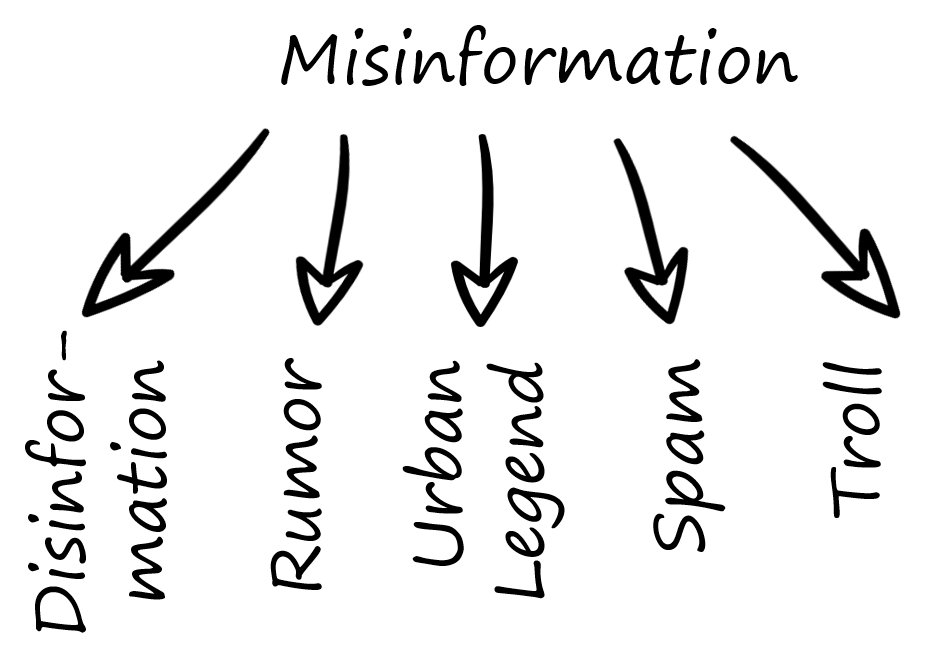
\includegraphics[width=4cm]{misinformation graphic.png}
    \caption{Misinformation Labels \citep{wu2016mining}}
    \label{fig:misinformation graphic.png}
\end{figure}


The dividing line between most of these categories is the level of intentionality: e.g. \textit{misinformation} is false but the creator has no verifiable  intent to mislead the reader, whereas \textit{disinformation} is false and the creator has a high intent to mislead the reader, and \textit{rumors} may be true or false, but the truth value is currently undetermined.

This has lead to an alternative definition from Klein \& Wueller: "[misinformation is] a news article that is intentionally and verifiably false". \citep{klein2017fake}. This definition has seen growth and has also been accepted by current studies \citep{shu2017fake, liu2018early}.

To bridge this gap, a more epistemological approach will be implemented. For every tweet $t$ in the set of tweets, there is a corresponding truth value $\tau$ between 0 and 1 (0 means something is completely false and 1 means something is completely true):
\begin{equation}
\label{truthvalues}
    \forall \ t \in T \ \exists \ \tau, \tau \in \mathbb{R} \ | \ 0 \leq \tau \leq 1
\end{equation}
Several previous works on this topic set $\tau \in \ \{0,1\}$ \citep{liu2018early,shu2017fake}. This is incorrect, as statements may be false, partially true, mostly true, or completely true. For example, this tweet from conservative provocateur Charlie Kirk (fig. \ref{fig:Charlie Kirk Tweet, May 4, 2020}) was rated "mostly false" by Snopes \citep{lee2020pelosi}: while Speaker Pelosi did say in an interview that she wanted to consider "guaranteed incomes" for Americans, including foreign workers without social security numbers \citep{pelosi2020maher}, she did not clearly define if "guaranteed income" meant the 2020 Paycheck Protection Plan (PPP) or something more akin to Universal Basic Income (UBI) as Kirk implies; she requested congress "consider it" and did not says she "wanted it"; both PPP and UBI would have directly affected \textit{all of} the 31 million Americans out of work rather than \textit{only} the undocumented immigrants as Kirk suggests. Therefore, since it is \textit{mostly} false but not \textit{completely} false, it would be unfair to say that $\tau_k = 0$ for this tweet; $ 0 < \tau_k < 0.5$ is more accurate. 
 \begin{figure}[htp]
    \centering
    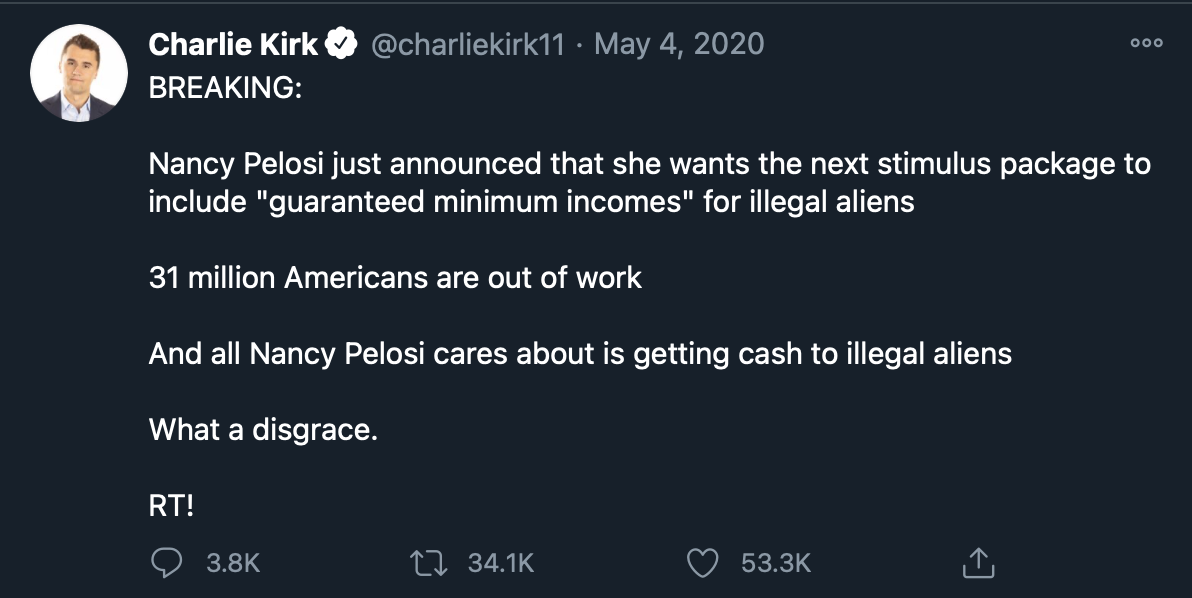
\includegraphics[width=11cm]{CharlieKirk Tweet.png}
    \caption{Charlie Kirk Tweet}
    \label{fig:Charlie Kirk Tweet, May 4, 2020}
\end{figure}



In another example, this tweet from Bernie Sanders is "mostly true": 
 \begin{figure}[htp]
    \centering
    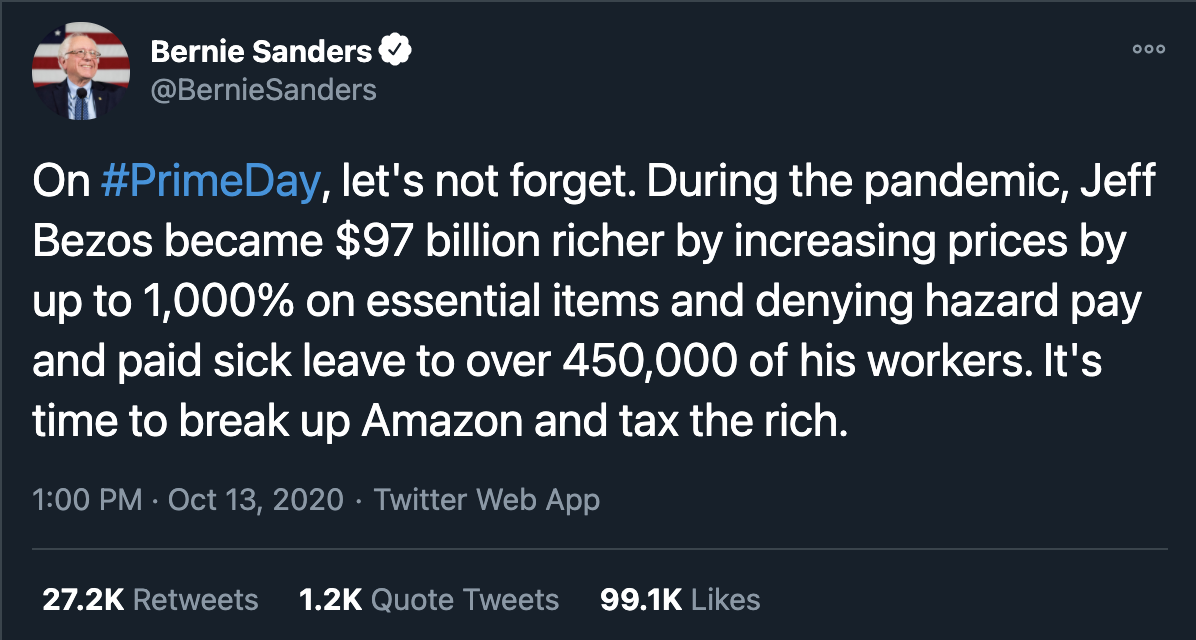
\includegraphics[width=11cm]{BernieTweet.png}
    \caption{Bernie Sanders Tweet}
    \label{fig:Bernie Sanders Tweet, Oct 13, 2020}
\end{figure}

While it is true that Amazon's employees have been denied hazard or sick pay (or have struggled with the mostly automated Amazon HR) \citep{cnbc2020amazon,guardian2020amazon}, and Jeff Bezos's wealth increased by almost 80\% during 2020 due to Amazon's 40\% increase in sales year over year for Q2 (and the majority of his wealth is tied to Amazon shares) \citep{Stebbins2020bezos}, other articles discussing the increase in price on essential items point out that this was mostly Amazon \textit{re-sellers} using the Amazon marketplace, not Amazon directly \citep{nicas2020sanitizer, kim2020price,gibson2020amazon}, Amazon banned over 6,000 of these price gougers \citep{bezos2020letter}, and that in cases where Amazon's price-generating AI had raised the price to an extreme level, it was returned to a reasonable level before Sen. Sanders wrote this tweet \citep{harman2020prime}. Therefore, it would not be reasonable to say that $\tau_s = 1$ for this tweet; it is $ 0.5 < \tau_s < 1$. 

Unlike with Charlie Kirk's tweet, which featured a single true sentence and many surrounding falsehoods, Senator Sanders's tweet has many true statements and one untrue (or at least misleading) statement, hence the rating of "mostly true". Much like how it was unreasonable to say $\tau_k = 0$ or $\tau_s = 1$, it is also unreasonable to say $\tau_k = \tau_s$. This nuance is meaningful and is not captured in the other literature. Therefore, an alternative solution to determining truth values must be used.

In \underline{Critique of Pure Reason} in 1781, Immanuel Kant proposed that statements should be broken into four groups: \textit{analytic a priori}, \textit{analytic a posteriori}, \textit{synthetic a priori}, and \textit{synthetic a posteriori} \citep{kant1908critique,frege1988collected,quine1951main}. \textit{Analytic} statements, per Kant, have the predicate contained in the subject, whereas \textit{synthetic} statements require a combination of understandings; \textit{a priori} statements are known without needing experience, whereas \textit{a posteriori} statements require experience to know if they are true \citep{wright1997companion}.
\subsection{Analytic a Priori}
An \textit{analytic a priori} statement's truth value is "true by virtue of meanings and independent of fact" \citep{quine1951main}. 
For example, proposition 1: \\$P_1$: All triangles have three sides.\\
The predicate "having three sides" is contained within the meaning of the word "triangle". There is no need to observe a given triangle in order to know that it must have three sides.

For the purposes of this discussion, racial slurs and other such language shall be considered \textit{analytic a priori} hate speech, as there is no need to observe all racial slurs in order to know that they were created and used with hate speech as the intent. Hate speech are fundamentally false statements \citep{waldron2012harm}, which automatically mean $\tau = 0$ .

\subsection{Synthetic a Priori}
A \textit{synthetic a priori} statement is true if it is universally true, no experience is needed to confirm it, but it is also not definitional in nature: \\
$P_2$: The sum of two sides of a triangle are greater than the third side. \\
As with $P_1$, there is no need to measure every triangle in existence to confirm this statement is true, yet there is nothing contained in the definition of a triangle that implies this relationship between the three sides.

In this thesis, spam will be considered false \textit{synthetic a priori} statements. Naive-Bayes classifiers have been incredibly successful at detecting spam messages \citep{wang2010detecting,xu2019exploiting,ahmed2018detecting}, in large part because they consistently illustrate the same telltale signs of being spam: broken English, seemingly random URL links, etc. Therefore, \\
$P_3$: Spam messages are unsolicited messages that feature broken English, random url links, etc. \\
$P_4$: Unsolicited messages that features broken English, random url links, etc. are not truthful \\
Leads to the conclusion that spam is not truthful, even though there is nothing in the definition of the word "spam" that leads to a truth value.


\subsection{Analytic a Posteriori}
A statement is \textit{analytic a posteriori} if it is true by virtue of its definition, but requires empirical evidence to discover it \citep{kripke1972naming}. Kripke gives the example of Venus being both the morning and evening star: \\
$P_5$: Venus is the morning star.\\
$P_6$: Venus is the evening star.\\
$C$: The morning star is the evening star.

While this statement is necessarily true based off of the definitions of "morning star" and "evening star", it can't be considered \textit{a priori} true, as Homer (12th century BCE) refers to the morning and evening stars as separate objects, and it isn't until Pythagoras (500 BCE) that it is a scientifically accepted fact that the morning and evening stars refer to the same object, Venus \citep{dunne1978voyage}.

Scientific information would largely fall into this category. Propositions such as: \\
$P_7$: Water is H$_2$O \\
are necessarily true and definitionally true, but were not known since the start of time -- in the case of water, it was not formally known until Avogadro in 1811. Scientific conspiracies such as the Earth being flat, would therefore be examples of \textit{analytic a posteriori} misinformation, as the Earth being round is scientifically true and definitionally true, per Frege, as any complete definition of the Earth would have to imply that it was a round planet \citep{frege2003sense}.

\subsection{Synthetic a Posteriori}
A statement is \textit{synthetic a posteriori} if its truth value is contingent upon experience and non-definitional in nature. Statements such as: \\
$P_8$: John Adams and Thomas Jefferson both died on July 4th, 1826\\
would be \textit{synthetic a posteriori} true statements, as they are objectively true, but there is nothing in the definition of "John Adams" or "Thomas Jefferson" that implies a death date. External verification is necessary in order to determine the truthfulness of the statement.

The majority of the statements that Wu et al. attempt to break into subgroups would all be considered \textit{sythentic a posteriori} statements here: rumors, legends, etc. may or may not be true, but require external validation in order to determine their truthfulness.

To summarize, with examples of misinformation according to each distinction: 
\begin{table}[h!]
    \centering
    \begin{tabular}{ |p{3cm}|p{5cm}|p{5cm}|}
    \hline
    & Analytic & Synthetic\\
    \hline
    A Priori & Hate Speech & Spam\\
    \hline
    A Posteriori &  Scientific Misinformation  & General Misinformation\\
    \hline
    \end{tabular}
    \caption{Misinformation Examples of Analytic/Synthetic Distinctions}
    \label{tab:misinformationexamples}
\end{table}


In terms of truth values, $\tau$, \textit{a priori} and \textit{analytic} statements are binary, but \textit{synthetic a posteriori} sentences may have a range of truthfulness (such as being misleading, partially true, mostly true, etc.):

\begin{table}[h!]
\centering
\begin{tabular}{ |p{3cm}|p{5cm}|p{5cm}|}
 \hline
  & Analytic & Synthetic\\
 \hline
 A Priori & $\tau \in\ \{0,1\}$ & $\tau \in\ \{0,1\}$\\
 \hline
 A Posteriori &  $\tau \in\ \{0,1\}$  & $\tau \in \mathbb{R} \ | \ 0 \leq \tau \leq 1$ \\
 \hline
\end{tabular}
\caption{Truth Values of Analytic/Synthetic Distinctions}
\label{tab:truthvalues}
\end{table}

These proposed distinctions better capture the breadth of misinformation than the previously provided definitions: as with Klein, it concurs that intentionality is not relevant in determining truth value; unlike Wu et al. or DiFonzo \& Bordia, it makes no distinction between types of misinformation such as "rumor" and "misinformation"; unlike Liu \& Wu, it separates hate speech, spam, and scientific misinformation from generalized misinformation. 

It is important not to separate rumor from misinformation as Wu et al. or DiFonzo \& Bordia do as rumors can be just as destructive. In the case of the 2013 Boston Bombing, members of social media hypothesized that an innocent Brown University student was behind the attack \citep{starbird2014rumors}; he committed suicide shortly after. Similarly, a father of a child who was killed during the 2012 Sandy Hook shooting committed suicide after being harassed by social media members convinced that the shooting was a hoax \citep{williamson2019alex}. More recently, on September 9th 2020, a conspiracy theory began that the fires in Oregon were started by the left-wing activist group called Antifa \citep{robinson2020oregon}. On September 11th, 2020, the FBI put out a statement declaring the reports untrue \citep{fbi2020portland}, and on September 12th, Facebook began removing these untrue posts. However, Oregon officials were so overwhelmed by calls and emails about this rumor that they had to waste resources that should have been going towards firefighting to handle them \citep{wilson2020oregon}. Wu et al. and DiFonzo \& Bordia would have called this claim a "rumor" from Sept 9th to Sept 11th, when it was officially debunked, yet even during that time period precious resources were being wasted. 
Clearly, rumors can have deadly consequences on par with general misinformation.

It also important to separate out hate speech, spam, and scientific misinformation from generalized misinformation. These are tasks that current machine learning is uniquely suited for, already have a great deal of available literature \citep{xu2019exploiting,wang2010detecting,ahmed2018detecting,al2019spam,oriola2020evaluating,gaydhani2018detecting,al2020lies,farrell2019evidence}, and which this thesis does not plan to improve upon. 

\subsection{Hyperbole, Sarcasm, and Irony}
Finally, hyperbole, sarcasm, and irony should be separated from our truth value set, as these are statements that are intentionally false to point to a greater underlying truth. 
Current literature on using NLP to decipher sarcasm and irony primarily revolves around unexpected word combinations \citep{barbieri2014modelling,buschmeier2014impact,ghosh2015sarcastic} or RoBERTa recurrent neural networks \citep{potamias2020transformer}, and they all examine publicly available data sets, namely the Riloff Twitter set \citep{riloff2013sarcasm}, the Pt{\'a}{\v{c}}ek Twitter set \citep{ptavcek2014sarcasm}, the Khodak Reddit set \citep{khodak2017large} and two "Semantic Evaluation Workshop Tasks" \citep{van2018semeval,ghosh2015semeval}. Many of these are able to generate quite high F1 scores, especially the RCNN-RoBERTa transformer proposed by Potomias, Siolas, and Stafylopatis, whose F1 score was consistently around 0.8 in each of the unique data sets. 

However, as Oprea and Magdy point out, tools that are successful in one data set struggle in other data sets. Models trained in the Riloff data set can generate an F1 score above 0.8, but those same models will generate an F1 score near 0.5 (which is the same as random guessing) when applied to the Pt{\'a}{\v{c}}ek set \citep{oprea2019exploring}. This implies there are extreme differences in how groups express and perceive irony/sarcasm/hyperbole. Those differences are beyond the scope of what RNNs and RCNNs can currently successfully grasp. Therefore an alternative solution to handling irony on a global level is necessary.

\section{Currently Implemented Solutions}
In all of the literature reviewed for this thesis on the topic fake news, there was very little if any time spent discussing the currently implemented solutions and their shortcomings. This thesis will try to rectify that and show why alternative solutions are needed in comparison to the status quo.

In his 2018 testimony to congress, Mark Zuckerberg agreed that the current process with content reviewers had room for improvement, saying "... unfortunately, with the amount of content in our systems and the current systems that we have in place to review, we make a relatively small percent of mistakes in content review but that is too many, and this is an area where we need to improve" \citep{energy2018facebook}, and then pivoted to discussing the need for AI solutions. In his 2020 testimony to congress, Zuckerberg stated that they had tripled the security team to 35,000 employees, that they're funding new security technologies to prevent emerging fake threats such as "deep fakes", and that they have implemented resource centers for hot button topics like COVID-19 and the 2020 election \citep{zuckerberg2020}.

\subsection{Current Solution per Facebook}
This section will look at Facebook's current solution, as it is more robust than Twitter's. Twitter currently only allows for flagging of political misinformation that is directly related to a political event, census, or impersonation (fig \ref{img:TwitterPolitics}:
\begin{figure}[htp]
    \centering
    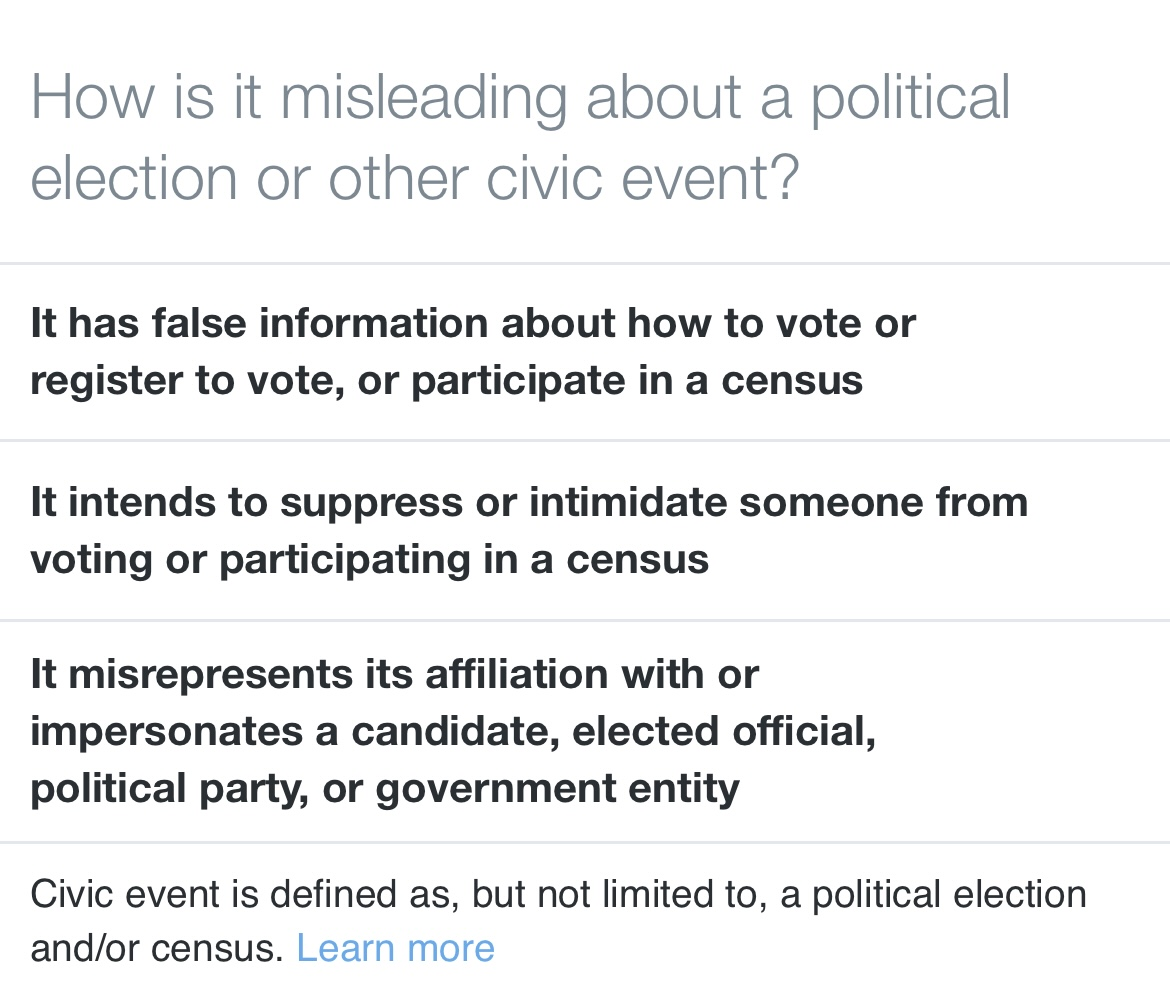
\includegraphics[width=6cm]{TwitterPolitics.jpg}
    \caption{Options for Flagging a Misleading Political Post on Twitter, Dec 2020}
    \label{img:TwitterPolitics}
\end{figure}

As Zuckerberg admitted in 2018, scale is an issue. Facebook currently has a preemptive solution and a two step solution:
\renewcommand{\labelenumii}{\Roman{enumii}}
\begin{enumerate}
\item The preemptive solution is to add a “context” button to all political posts, which a user can click on for more information \citep{smith2018designing}.
 \item If a post has been shared and is untrue, the following steps must be taken before Facebook will flag a post as false:
 \begin{enumerate}
     \item It requires an outside individual to report the post. 
     \item After the post is reported, then it is  sent to 3rd-party fact checkers for verification. 
     \item Third party fact checkers must log in to the Facebook dashboard and then provide a link proving the story is false (they cannot simply mark a story as untrue).
 \end{enumerate}
 \end{enumerate}
 
 In Facebook’s case, after they have determined a particular post is false, then the post is shown less frequently (80 percent less), other posts of the same link or image will also be shown less, it will be unable to be converted into an ad later, and someone re-sharing this post will be given a notification that the information is likely false \citep{owen2016clamping,facebook2020fact}.
 
 The punishment for routine offenders or for routine fake stories that point to a common domain is a loss of advertising rights and a loss of ability to monetize \citep{facebook2020fact}.
 
 
 
 \subsection{Issues with Preemptive Solution}
 The "context" button is ineffective for several reasons. 
 
 First, it assumes that people will actively search for context when viewing a link. People are unlikely to feel the need to do further research if they agree with or believe the headline as presented \citep{nyhan2010corrections}. This problem is augmented by the fact that headlines are often misleading and written to draw the strongest possible emotional response \citep{chesney2017incongruent,ecker2014effects,bell1984good,molek2013towards,kilgo2018new,vettehen2008explaining}. For example with the \textit{Express} newspaper from the UK (from Ecker, et al.):
 \begin{itemize}
 \item Headline: Air pollution now leading cause of lung cancer
\item Evidence within article: “We now know that outdoor air pollution is not only a major risk to health in general, but also a leading \textbf{environmental} cause of cancer deaths.” Dr. Kurt Straif, of IARC [emphasis added]
 \end{itemize}
 
 Or from the \textit{Independent}'s Facebook page \citep{chesney2017incongruent}:
 \begin{itemize}
\item Social media post copy: Enjoy it while you
can
\item Social media headline \footnotetext[1]{https://www.facebook.com/TheIndependentOn-line/posts/10154972799736636}\footnotemark[1]: Scientists have predicted the end of sex
\item Article headline\footnotemark[2]\footnotetext[2]{Will Worley (2016): http://www.independent.co.uk/news/science/sex-unnecessary-designer-babies-stanfordprofessor-says-a6957636.html}: Sex will be made unnecessary by ‘designer babies’, professor says
\item Evidence within article: Professor Henry Greely believes that in as little as 20 years, most children will be conceived in a laboratory, rather than through sexual intercourse.
 \end{itemize}
 
 While there have been attempts to track down misleading headlines, they have primarily centered around \textit{click-bait} or tabloid headlines \citep{chen2015misleading,chakraborty2016stop} that require the user to click to find out the information, i.e. "Here’s What Happens When You Put A Few Little Kids In A Room With 2 Dolls In 2 Different Colors" \citep{chen2015misleading}. While this will help with some problems, both the \textit{Express} and \textit{The Independent} articles would not be caught by the proposed algorithms. 
 
 
Given that only 59\% of all shared URLs are ever clicked on Twitter \citep{gabielkov2016social} and there is clear evidence of misleading headlines, Twitter added in a feature that prompts users to read articles rather than just headlines before sharing the article \citep{reuters2020article}. Unsurprisingly, the backlash was immediate (fig: \ref{fig:House Judiciary GOP Tweet}):
 \begin{figure}[htp]
    \centering
    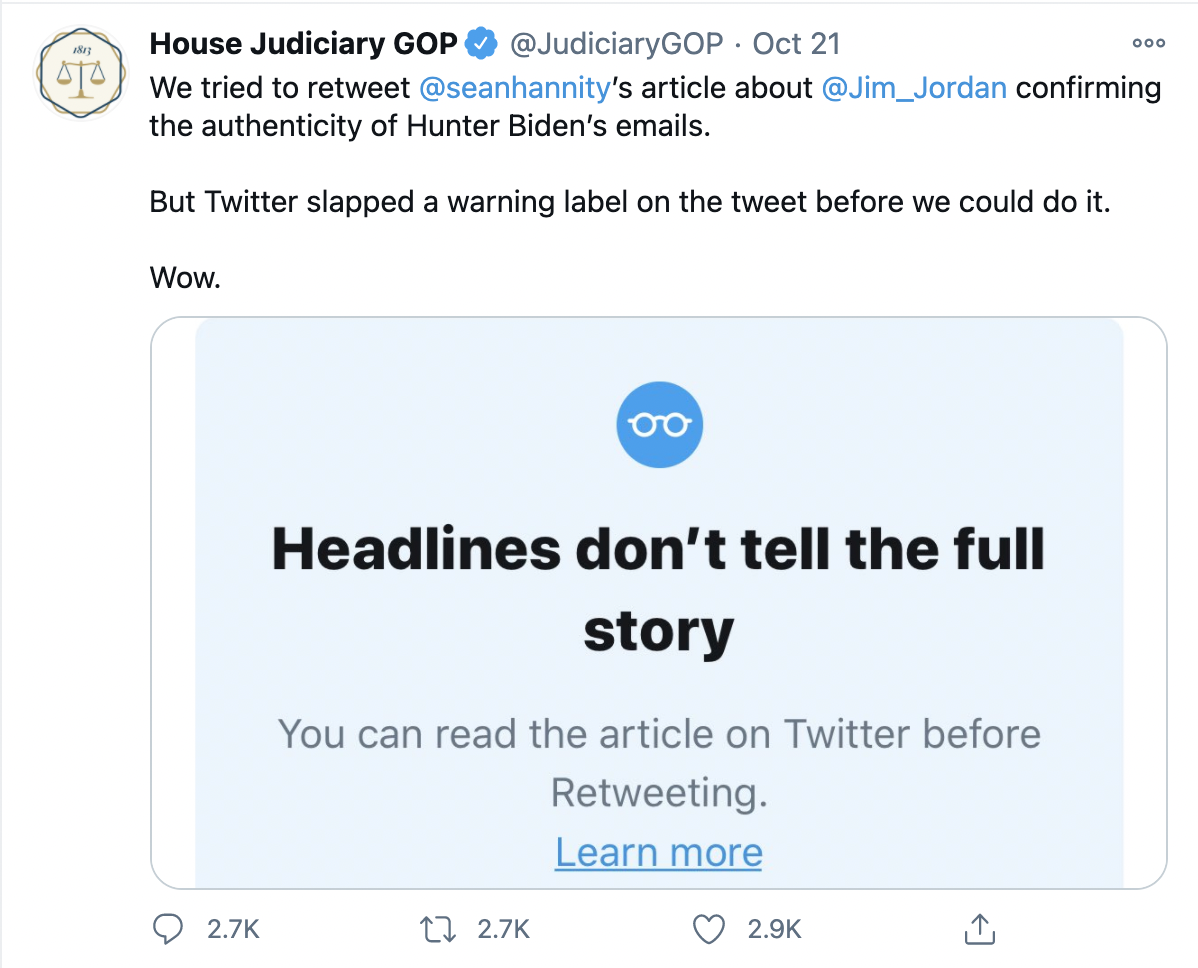
\includegraphics[width=8cm]{JudiciaryTweet.png}
    \caption{House Judiciary GOP Tweet}
    \label{fig:House Judiciary GOP Tweet}
\end{figure}

As will be discussed shortly, this fits the problem of \textit{echo chambers} wherein the primary question is not "is this correct" but "does it align with the views of my network?" 

To summarize, the proposed preemptive solution is ineffective because:
\begin{itemize}
\item 41\% of the time, someone will retweet an article without having read more than the headline. \citep{gabielkov2016social}
\item Headlines are written to be intentionally misleading, or at least to generate a strong emotional response from the reader.\citep{chesney2017incongruent}
\item Readers are unlikely to fact-check, question, or feel compelled to do outside research on an article if the have a strong emotional response to it.\citep{nyhan2010corrections}
\item Blanket warnings without explanation are likely to generate backlash \citep{reuters2020article}
 
 \end{itemize}
 \subsection{Issues with Two Step Solution}
 The key first step for this solution is that an individual must report the post as false. This requires a level of self policing that it is unlikely given the prevalence of \textit{echo chambers}. 

Because social media seeks to connect like minded individuals, it has a tendency to generate \textit{echo chambers}, or closed networks with high repetition of content and low diversity of thought \citep{adibi2005proceedings, bastian2009international, pariser2011filter,bozdag2015breaking}. While not every closed homogeneous network is inherently bad -- they can operate as self-help groups \citep{kast2012under} or can encourage positive behavior like reducing prejudice \citep{paluck2011peer} -- there is a clear and well documented history that people are influenced by others in their network \citep{cialdini2004social,bollinger2012peer, bond201261,gerber2008social,gerber2009descriptive,meer2011brother,paluck2012salience,del2016spreading,bessi2015viral} and this can be destructive in the context of misinformation. For this paper's purposes, partisanship $\rho$, is defined as being on a scale of 0 to 1 with 0 being extremely left-wing and 1 being extremely right wing (a normalized version of most one-dimensional scales of the topic):
\begin{equation}
\label{basepartisanship}
    \forall \ u \in U \ \exists \ \rho \in \mathbb{R} \ | \ 0 \leq \rho \leq 1
\end{equation}
From here, $\rho_k$, the partisan leaning of some unique user $u_k$ is directly proportional to the partisan leaning of the \textit{echo chamber} network $n_n$ and can be described as follows:
 \begin{equation}
    \label{ech chamber}
        \langle \rho_n \rangle = \frac{1}{|n_n|}\sum_{i=1}^{|n_n|}{\rho_i}, (u_i \in n_n, n_n \in N)
 \end{equation}
 \begin{equation}
    \label{leaningproportionaltonetwork}
        \rho_k \sim \langle \rho_n \rangle
 \end{equation}
 
 For validation of this, in Asch's classic experiment, he found that individuals will conform to the opinions of the rest of the group, even if it runs contrary to their personal convictions \citep{asch1956studies}. For a more recent political example, in Bullock's experiments he found that participants would change their opinions on a particular topic if they were told that the party they identify with held an opposing view, even if it was counter-intuitive, such as a Republican being told that the Republican party was against a conservative initiative \citep{bullock2007experiments}. Other research provides similar results: Republicans and Democrats are likely to accept a statement as being true and not feel the need to research personally if it comes from a preferred politician \citep{housholder2014facebook}; even if a preferred politician's statements are disproved, there is no shift in voting intentions, party identification, or overall perceived credibility of that politician \citep{swire2017processing}. 
 
This provides a perfect opening for malicious actors, as they are primarily focused on sharing and inflaming hyper-partisan and extreme views \citep{bastos2019brexit,hegelich2016social}, such that the partisanship of a malicious actor, \textit{m}, from the set of malicious actors, \textit{M}, will be extreme: 
\begin{equation}
\label{trollpartisanship}
\forall \ m \in M, \exists \ \rho \in \{0,1\}.
\end{equation}

Mirroring viral spread seen in other scale-free network analyses \citep{pastor2001epidemic,cohen2003efficient}, this problem quickly escalates: for every network that has an an average partisanship $\langle \rho \rangle$ approximately equal to the target partisanship of the malicious actors $\rho_m$, the number of malicious actors, \textit{m}, will increase:
\begin{equation}
\label{maliciousactorsincreasenetwork}
    n \in N, \langle \rho \rangle \sim \rho_m: |u \in n| + m > |u \in n|
\end{equation}
As \textit{m} increases, the group partisanship will shift towards the \{0,1\} binary from equation \ref{trollpartisanship}: 
\begin{equation}
\langle \rho \rangle \rightarrow \rho_m \in \{0,1\}
\end{equation} 
And given Bullock's experiments and equation \ref{leaningproportionaltonetwork}:
\begin{equation}
\label{peopletoextremes}
    \forall u \in n: \rho \sim \langle \rho_n \rangle: \rho \rightarrow \rho_m
\end{equation}
Equation \ref{peopletoextremes} correlates perfectly with the social experiments by Asch and Bullock mentioned previously, and more recent research has confirmed these findings \citep{colliander2019fake,edelson2011following}. Even when the groups were anonymous users on the internet, users will still be motivated by a desire to conform to the group's opinions and, if necessary, relinquish their own previous beliefs  \citep{williams2000cyberostracism,zhu2012switch,tsikerdekis2013effects,breitsohl2015groupthink,winter2015they,hamilton2017s}. 

The closer $\langle \rho \rangle$ gets to 0 or 1, the more closed the network becomes, and the more resistant to fact-checking or corrective information coming from outside of their network \citep{garrett2013undermining,lord1979biased,edwards1996disconfirmation,redlawsk2002hot, taber2006motivated}. This explains both why even the release of President Obama's long form birth certificate only briefly subdued the conspiracy that he was not born in the United States \citep{nyhan2012new} and why the Pizzagate conspiracy discussed earlier lived even after it had been disproved months earlier -- so long as the corrective information came from outside of the echo-chamber, it was fundamentally dismissed.


\subsection{Partisanship} 
There is substantial research that Americans who identify as right-wing have historically been more susceptible than other subsets of the American population to fake news \citep{guess2019less,benkler2018network,grinberg2019fake,allcott2017social,badawy2018analyzing}, but more thorough analysis suggests that this pattern may not hold up moving forward.

First, there may be an over representation in terms of conservative vs. left misinformation in the analyzed data sets. In the Russian troll data set provided by Twitter, there were twice as many right leaning trolls as left leaning trolls \citep{freelon2020black,badawy2018analyzing,benkler2018network}. It is likely that this is a positive feedback loop: since conservatives were more likely to consume fake news, there were more trolls creating fake content for them, which they in turn would be more likely to share \citep{bakir2018fake,bodo2019interested,silverman2016analysis,pariser2011filter}. 


Second, a better predictor of willingness to share misinformation is general distrust in the media rather than political leaning \citep{hopp2020people,shin2017partisan,kahan2012ideology,lewandowsky2016motivated,swire2017processing,mourao2019fake}. This is further born out by the Russian "troll farm" known as the Internet Research Agency (IRA) heavily targeting two groups they determined were unlikely to trust the main stream media: far right-wing Americans and Black Americans \citep{diresta2019tactics,howard2019ira,boatwright2018troll,jamieson2020cyberwar,mueller2019mueller,freelon2020black}. In fact, the IRA spent a disproportionately high amount in micro-targeting Black Americans and generated a high return on their investment (the average misinformation post targeted at a Black American was 2.5 times more likely to receive an engagement, such as a like or retweet, from a real user than a misinformation post targeted at a general conservative American) \citep{howard2019ira,freelon2020black}.

Third, many of sharers of misinformation are more focused on empathy with a particular group \citep{winter2015they,rheault2016measuring,dale2017nlp} or engaging in signaling theory with a group \citep{connelly2011signaling,lampe2007familiar,spence2002signaling} rather than objective truth. Dominic Cummings callously stated while creating inaccurate content for the Leave campaign for Brexit that "accuracy is for snake-oil pussies" \citep{crace2016accuracy}, yet his point is widespread and in line with the analysis of \textit{echo chambers}: in hyper-partisan situations, strongly held opinions that are counter to widely accepted narratives are seen primarily as signals of commonality \citep{yla2018populist,noppari2019user,lazer2018science,yla2019politicization,wasilewski2019us,freelon2020russian}. 


Fourth, there is no difference in propensity to share non-partisan misinformation, such as the dangers of living near power lines, the side-effects of MMR vaccines, or the safety of nuclear power reactors between people of various beliefs \citep{kahan2015climate,hara2016co,kahan2012ideology,lewandowsky2016motivated,barbera2015tweeting}.

Finally, most of the studies referenced previously looked at data from 2015/2016 and before. Since 2015, there has been a well documented global rise in populism on the left end of the spectrum to match the rise on the right that had previously existed and was documented earlier. For example, there was a 33x increase in membership in far-left organizations such as the Democratic Socialists of America between 2015 and 2020 \citep{godfrey2020thousands}, left-leaning populist groups in France saw outsized social media volume in the 2017 elections \citep{donadio2017french}, and the U.K's Labour party took a shift to the populist left under the leadership of Jeremy Corbyn starting in 2015 \citep{wainwright2018remarkable,hobson_fielding_2019}. This leftward shift can be statistically seen in the United States Congress by comparing the voting patterns of the 115th (Jan 2017 - Jan 2019) (fig. \ref{fig:115th House}) and 116th (Jan 2019 - Jan 2020) (fig. \ref{fig:116th House}) House of Representatives \citep{fivethirtyeight2018tracking}. In both of these illustrations, Democrats are blue, Republicans are red, Independents are orange, and the scale for each Representative is the same $0\leq \rho \leq 1$ scale seen in equation \ref{basepartisanship}. Here, a representative who always voted in line with President Trump's position has $\rho = 1$, and someone who never voted in line with President Trump has $\rho = 0$:

 \begin{figure}[h]
\minipage{0.5\textwidth}
  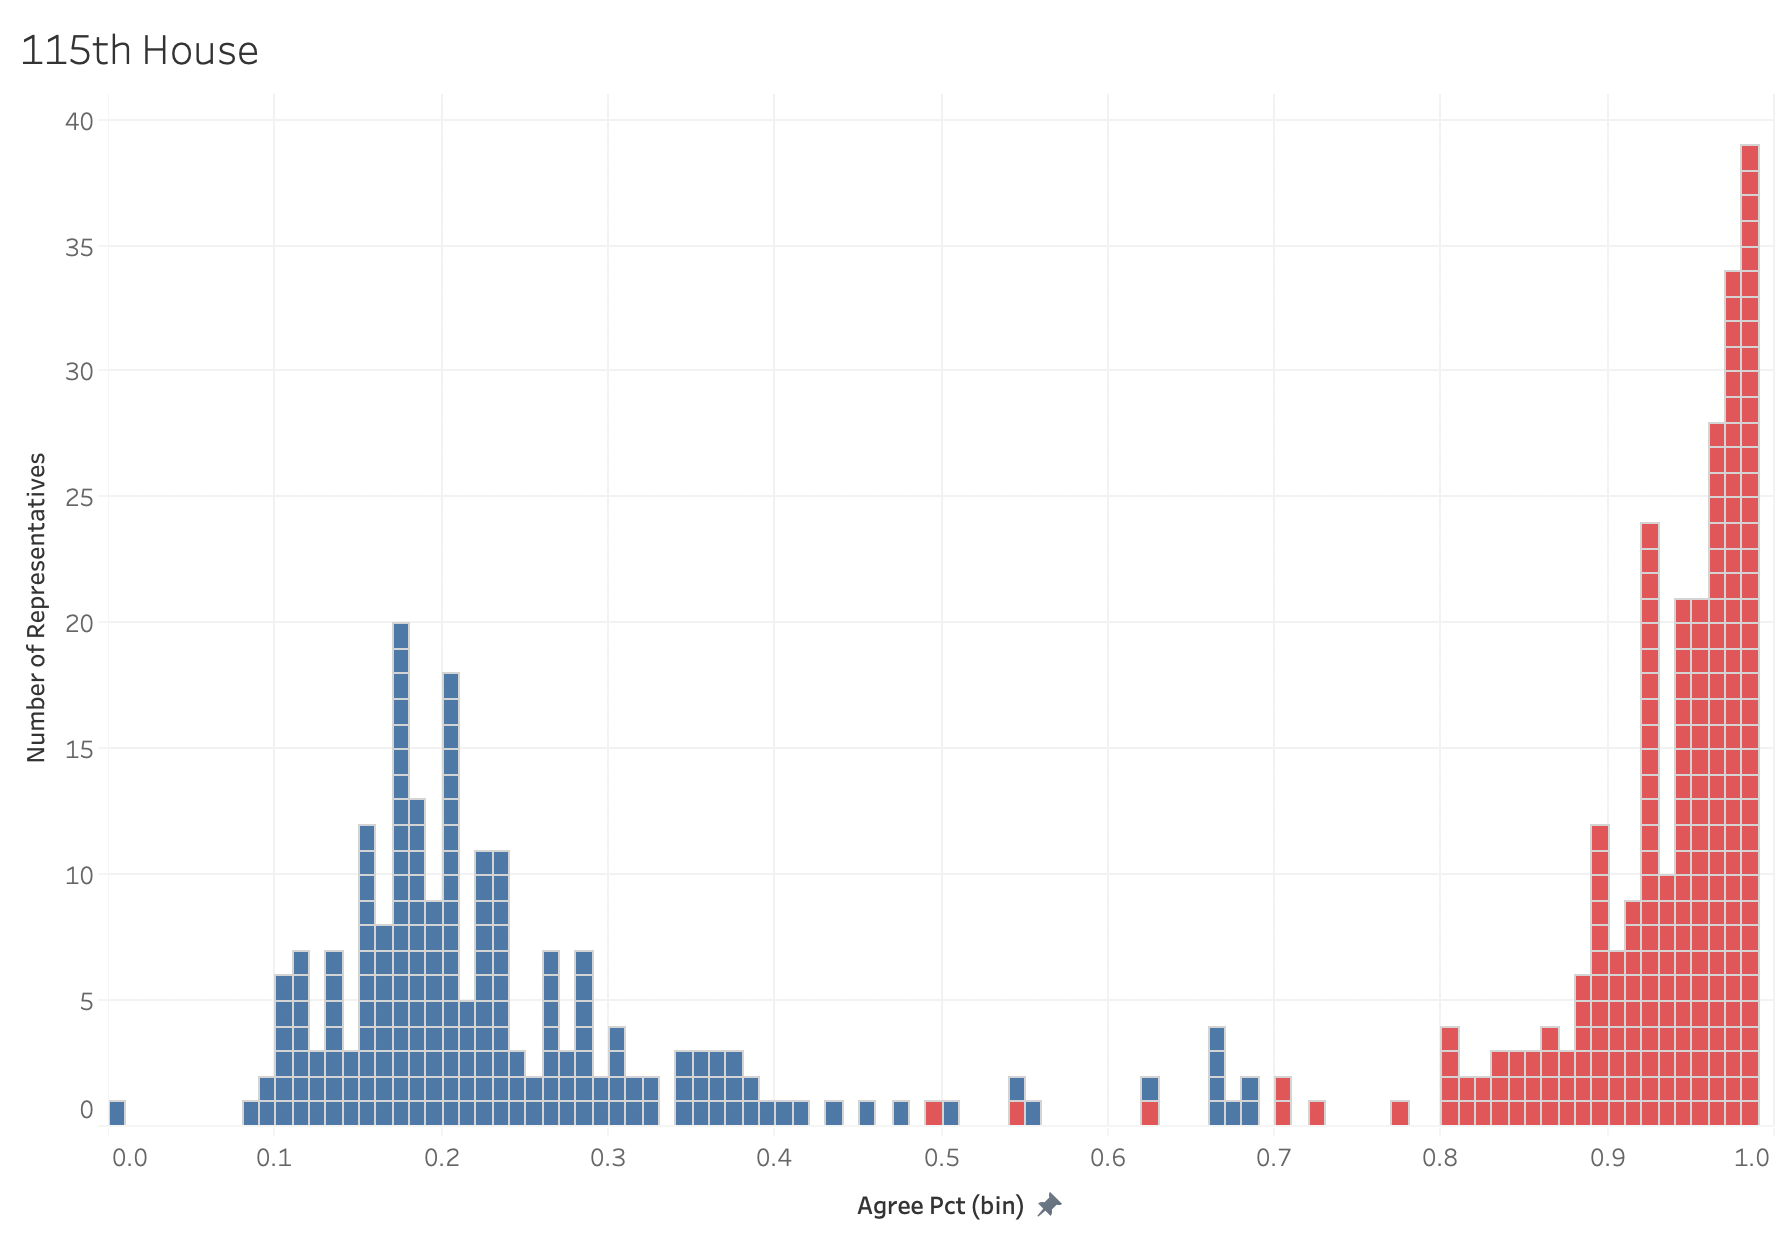
\includegraphics[width=\linewidth]{115th House.png}
  \caption{115th House of Representatives}\label{fig:115th House}
\endminipage\hfill
\minipage{0.5\textwidth}
  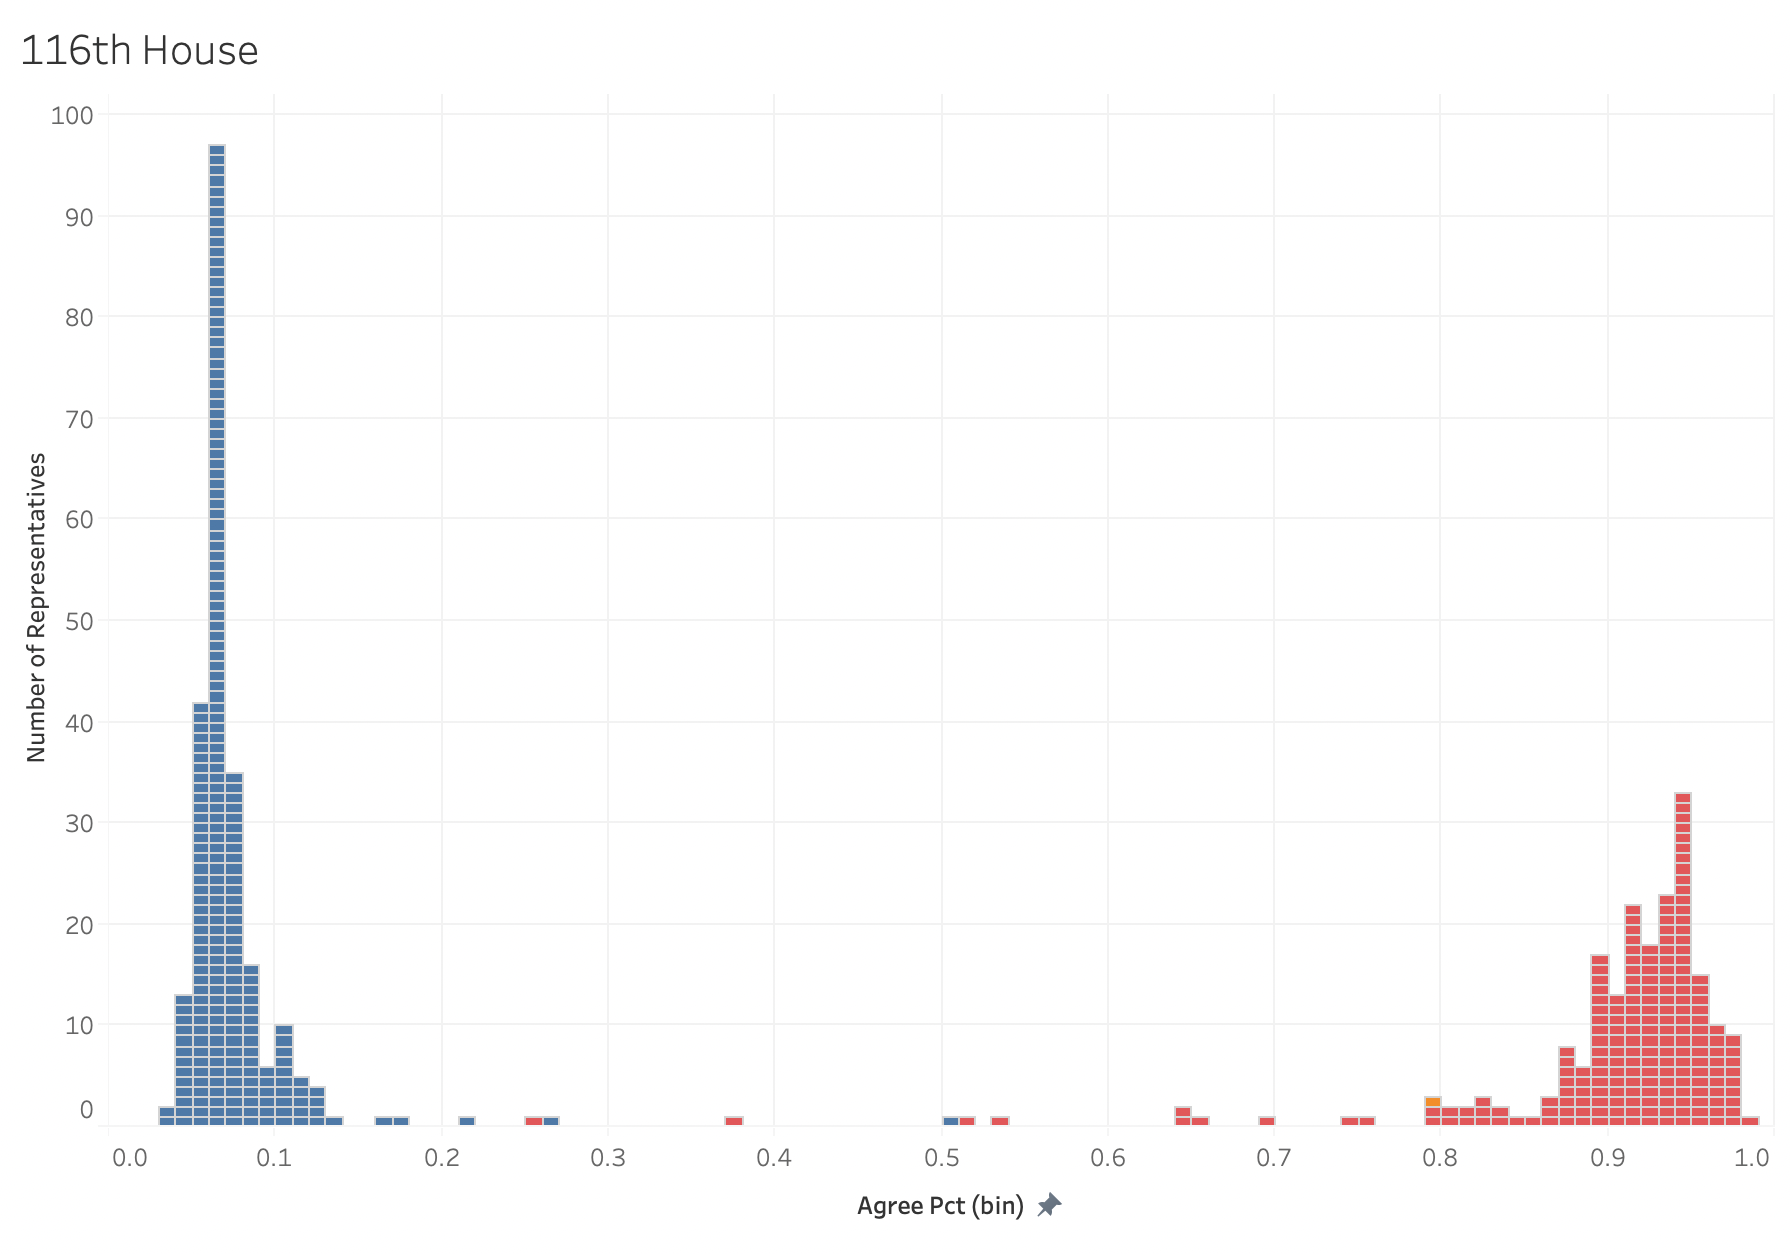
\includegraphics[width=\linewidth]{116th House.png}
  \caption{116th House of Representatives}\label{fig:116th House}
\endminipage\hfill
\end{figure}
 
 In the 115th congress, Republican members had an average $\langle \rho_r \rangle = 0.93$ and Democratic members had an average $\langle \rho_d \rangle = 0.24$. In the 116th congress, Republican members had an average $\langle \rho_r \rangle = 0.91$, Democratic members had an average $\langle \rho_d \rangle = 0.08$, and Independent members had an average $\langle \rho_i \rangle = 0.79$. While the Democratic party did pick up +40 seats in the 2018 midterms, simply adding or subtracting members does not imply a shift in partisanship as the Republican partisanship barely changed between the 115th and 116th Congress. For the state of Pennsylvania, which very narrowly broke for President Trump in 2016, the Democratic members had a $\langle \rho \rangle = 0.39$ in the 115th Congress and a $\langle \rho \rangle= 0.07$ in the 116th.
 
 For comparison, the US Senate is somewhat more stable, possibly beacause Senators are only up for election every 6 years instead of every 2, so turnover is less frequent. In the 115th congress, Republican senators had an average $\langle \rho_r \rangle = 0.91$, Democratic senators had an average $\langle \rho_d \rangle = 0.30$, and Independent senators had an average $\langle \rho_i \rangle = 0.30$. In the 116th congress, Republican senators had an average $\langle \rho_r \rangle = 0.83$, Democratic senators had an average $\langle \rho_d \rangle = 0.19$, and Independent senators had an average $\langle \rho_i \rangle = 0.22$.
 
 As illustrated before, a shift in the average partisanship of the network towards the \{0,1\} binary strongly correlates to populism and a susceptibility to misinformation \citep{hopp2020people,kahan2012ideology,mourao2019fake,shin2017partisan,swire2017processing,vargo2018agenda}. This can already been seen anecdotally, as there has been an uptick in left-leaning misinformation (or hyper-partisan opinions counter to the general accepted facts, per point two of this section)  since 2018, including information around a confrontation between MAGA-hat wearing teenagers, Black Israelites, and a Native American elder at the Lincoln Memorial in 2019 \citep{sacks2019maga,healy2019believing,pond2020complexity}, and the death of Breonna Taylor in 2020 \citep{duvall2020fact,kim2020fact}. 

 \subsection{Third Party Fact Checkers}
 The usage of third party fact checkers has two fundamental issues.
 
 First, there is a large volume of research over decades that ideologues on either side of the political spectrum will view the exact same content as being biased against them \citep{arpan2003experimental,baum2008eye,christen2002hostile,gunther2001predicting,gunther2004mapping,baum2004issue,gussin2004eye,lee2005liberal,vallone1985hostile}. This extends to fact-checking, as groups on both the left and the right post about claims of censorship when their content is removed or their reach is reduced \citep{Dreyfuss2020Now,Post2020Facebook,Millhiser2018Facebook}. 
 
 As Shin and Thorson note, however, closed networks are eager to fact check members who are not of their group. In 2018, Think Progress (a liberal Facebook fact checker) had an article on the Brett Kavanaugh Supreme Court confirmation hearing that was flagged as false by The Weekly Standard (a conservative Facebook fact checker) \citep{owen2018with}. Think Progress stated that then-Judge Kavanaugh had said during his hearing that he would kill Roe v. Wade \citep{millhiser2018brett}, a claim that was deemed false by the Weekly Standard and by FactCheck.org, a non-partisan fact-checking organization \citep{gore2018kavanaugh}. The Weekly Standard offered to remove its flag if Think Progress replaced the word "said" in the headline, as Judge Kavanaugh had not explicitly said that he would overturn Roe v. Wade. Think Progress argued that secondary and tertiary definitions of "said" made their headline correct, and instead accused Facebook of bias and censorship \citep{legum2018tweet}. Shortly after, several other liberal journalists made the same argument of censorship with none touching on whether or not the word "said" was truthful \citep{froomkin2018tweet,grim2018tweet,beutler2018tweet}. 
 
 This example matches the previous analysis of strongly held partisan views being "truer" than objective truth. It also aligns with other research that shows that closed groups are more than eager to fact-check individuals who do not belong to their group, such as Republicans fact checking Democrats and vice-versa \citep{shin2017partisan,iyengar2015fear}, and that they are unable or unwilling to recognize potential mischaracterizations of opposing viewpoints \citep{pennycook2019lazy,vargo2018agenda}. 
 
A better solution, clearly, would be only to use high quality non-partisan fact checkers, as they would be able to rise above the echo chamber issues. However, these well-regarded apolitical fact checkers, such as Snopes and the Associated Press, have either left their fact checking partnership with Facebook or stopped actively working. They argue that Facebook's process is manual, time consuming, ineffective, and does not provide adequate compensation for the time required to do the job thoroughly \citep{green2019message,coldeway2019update}. An ideal solution, then, most be one which limits the amount of time-consuming manual work, hence Zuckerberg's initial comments about AI being the key to solving this problem.

\subsection{Issues with Punishment}
By this point, it should be clear that the punishments imposed by Facebook are not effective, as they only seek to limit ad revenue and the ability to monetize. This implies a financial incentive for purveyors of incorrect information where, as has been shown, much of this is ideologically driven \citep{allcott2017social}. While these may be effective deterrents for the \textit{click-bait} or tabloid style headlines discussed earlier  \citep{chen2015misleading}, less than 0.1\% of traffic to fake news websites during the 2016 election came from paid media/advertising \citep{albright2016election2016}. 

The other key punishment that Facebook implements is on the actual post level. Posts deemed false are shown 80\% less frequently, and other posts showing the same link or image will also be shown less frequently. While this sounds promising, there is a fundamental flaw that can be exposed by examining Facebook's most recent papers on computer vision. Facebook's AI is a Convolutional Neural Network (CNN) \citep{carion2020end}, which is very good for detecting something in common across several images, such as a person's face \citep{kalinovskii2015compact}, but is easily fooled by changing parts of the image, such as adjusting font and colors, cropping, adding filters, etc \citep{sumbaly2020using}.

For example, this shutterstock image of Donald Trump (fig. \ref{fig:Trump Shutterstock Image}): 
 \begin{figure}[htp]
    \centering
    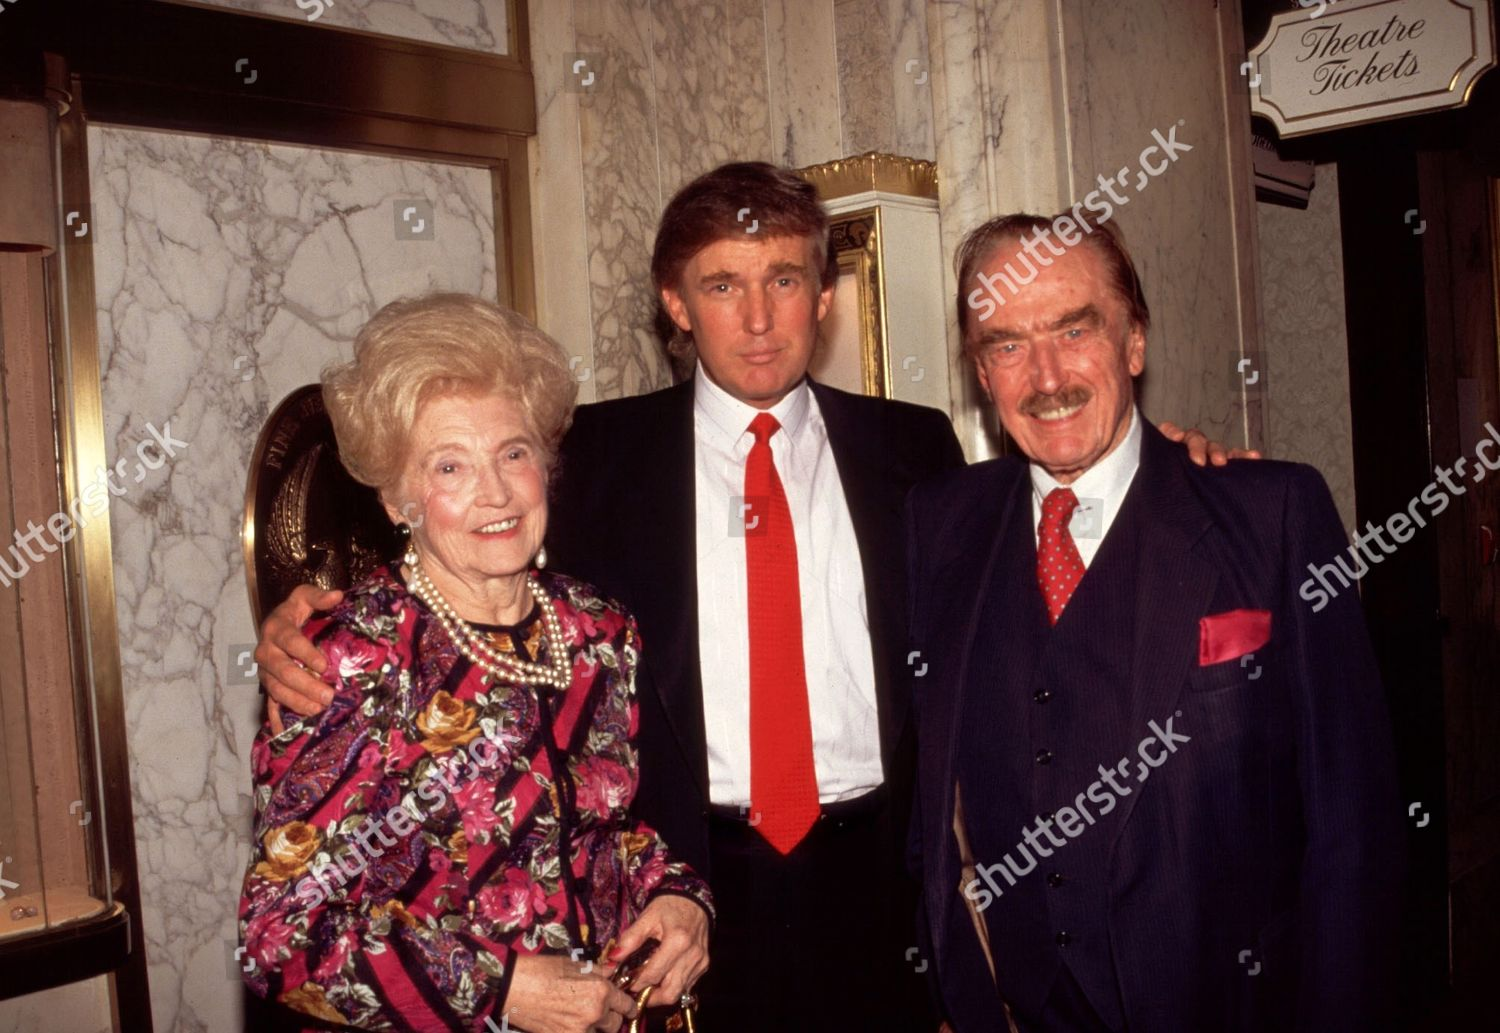
\includegraphics[width=8cm]{trumpkkk0.jpg}
    \caption{Trump Shutterstock Image}
    \label{fig:Trump Shutterstock Image}
\end{figure}

was photoshopped to make it appear as though his parents were wearing KKK robes. Reuters provided three different examples of the image that were widely shared on social media \citep{reuters2020trump} (Figures \ref{fig:TrumpKKK1}, \ref{fig:TrumpKKK2}, \ref{fig:TrumpKKK3}).

 \begin{figure}[h]
\minipage{0.32\textwidth}
  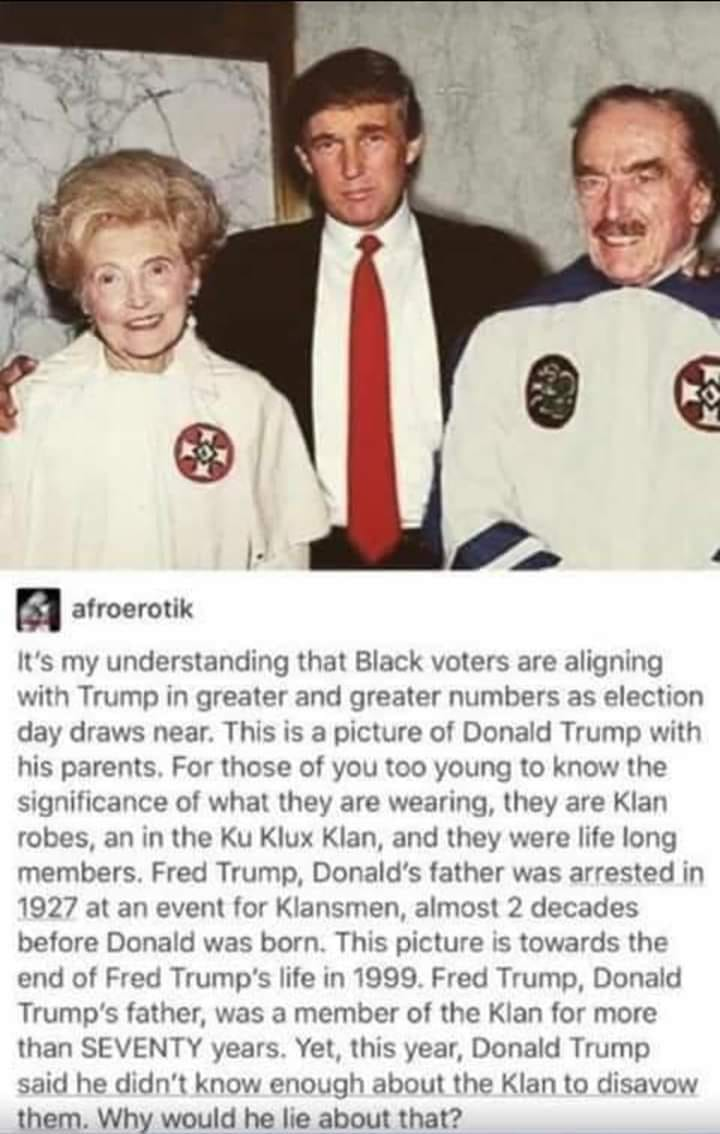
\includegraphics[width=\linewidth,height = 9cm]{trumpkkk1.jpg}
  \caption{Version 1 of Edited Trump Image}\label{fig:TrumpKKK1}
\endminipage\hfill
\minipage{0.32\textwidth}
  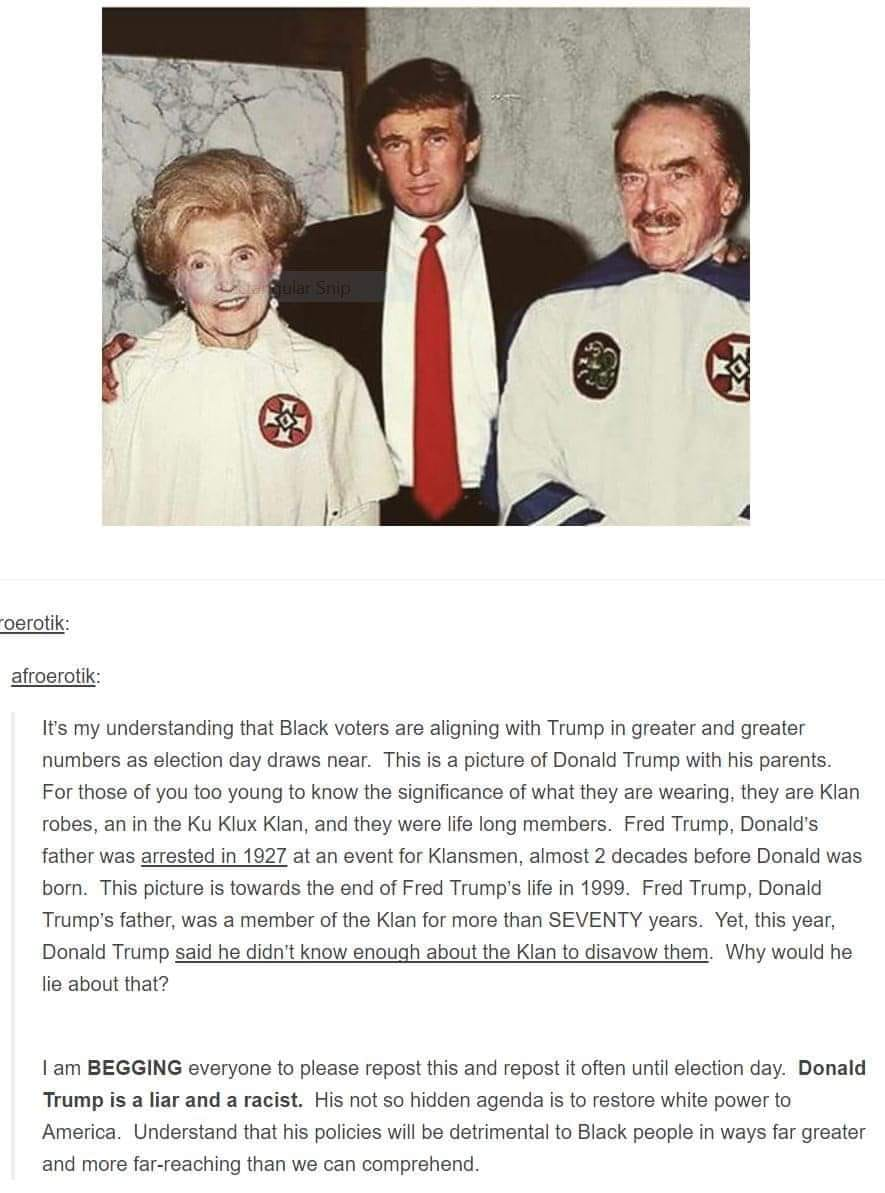
\includegraphics[width=\linewidth,height = 9cm]{trumpkkk2.jpg}
  \caption{Version 2 of Edited Trump Image}\label{fig:TrumpKKK2}
\endminipage\hfill
\minipage{0.32\textwidth}%
  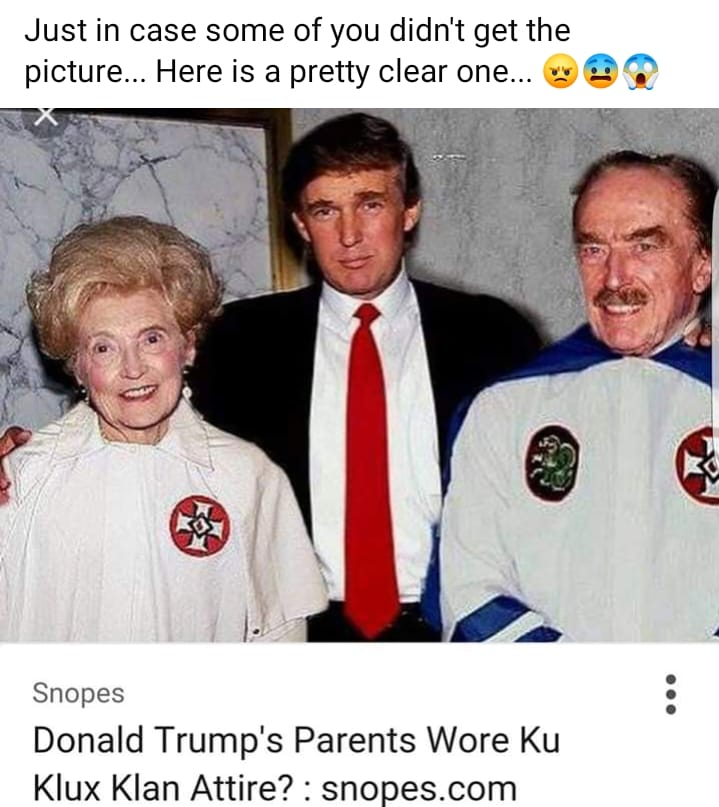
\includegraphics[width=\linewidth,height = 9cm]{trumpkkk3.jpg}
  \caption{Version 3 of Edited Trump Image}\label{fig:TrumpKKK3}
\endminipage
\end{figure}


To a human, all three of these images are roughly the same, but there is sufficient distorting in each image (e.g. some have removed pieces of the "shutterstock" watermark, others all of them; sections of the images have been cropped or stretched or mirrored; colors have been adjusted; etc.) combined with the variations in the text around the image to confuse a CNN. Facebook even admits that their CNN struggles to tell the difference between near-identical images and that there could be "thousands or millions of copies" of these undetected near-duplicates of already flagged content \citep{sumbaly2020using}. Their new solution, "SimSearchNet", is built specifically to solve this issue, but it is not fully effective yet. Avaaz, an activist organization with a focus on stopping the spread of fake news, found that 42\% of the misinformation content they analyzed in October was currently circumventing Facebook's policies. Even more disheartening, they were able to identify 738 posts that were not labeled as fake, in spite of having already been debunked, and had collectively racked up 5.6M interactions and 142M views \citep{schott2020brief}.

Some of these had the potential to influence the 2020 election, in spite of the extra measures Facebook and Twitter added \citep{dean2020facebook}: "While Facebook applied a contextual label to one false claim on a purple background about extra postage being required for mail-in ballots, another identical claim ran against a blue background with no intervention from Facebook. The former received 14,000 shares; the latter received 20,000" \citep{Fung2020facebook}.

Ultimately, neither of the proposed Facebook punishments are effective: reducing the ability to monetize is irrelevant for an ideological actor, and reducing the spread of an image or removing it entirely is insufficient if the same image can be recreated and re-shared so easily.

\subsection{Scale}
The issue of scale is not only non-trivial, but is unmentioned in the other literature on solving this issue. Attempting to crawl through every tweet and every URL posted would be an incredibly difficult task given that Facebook alone has 1.8 billion daily active users as of their Q3 2020 earnings report, with 2.54 billion daily active users of at least one tool in the Facebook portfolio (Facebook, Instagram, WhatsApp, etc.), with those numbers ballooning to 2.74 and 3.21 billion on a monthly level \citep{facebook2020q3}. Given that in 2014 Facebook generated 4 petabytes of data daily and ran 600,000 queries with 1 million map-reducing jobs when their total daily active users was 890 million \citep{bronson2015open}, a simple ratio would provide a conservative estimate that Facebook now generates at least 8.1 petabytes of data every day, with 1.2 million queries and 2.1 million map-reducing jobs. 

Many of the proposed solutions for fake news detection are RNN based, however RNNs are far too resource heavy to be successfully implemented at the necessary scale \citep{gehring2017novel, sze2017efficient}. Even transformer based attention models, like the ones suggested in the 2017 Facebook article on machine learning, require high amounts of compute power and primarily excel at tasks like language translation \citep{vaswani2017attention}. The detection of fake news is a more complex task, as a solution most not only decipher the language being used, but also interpret a representative truth value, and return a remove/don't-remove decision within a matter of hours of the initial post's timestamp, $p_i$.

As Facebook's digital footprint grows, a successful solution must be able to grow with it. 

\subsection{Summary}
To summarize, the current solution and issues are:
\renewcommand{\labelenumii}{\Roman{enumii}}
\begin{enumerate}
\item The preemptive solution is ineffective because users will not seek extra context
\begin{itemize}
\item Users will not seek extra context and will reject being prompted to look for extra context
\end{itemize}
\item An outside individual must report the post for further actions
 \begin{itemize}
     \item Users are unlikely to report posts that are in line with their partisan views
     \item Individual partisanship is strongly influenced by the beliefs of their network, which can be infiltrated by extremist ideology
     \item Extremist ideology on either side of the political spectrum is strongly resistant to fact checking, and maintaining beliefs that are opposed to generally accepted facts can actually be seen as proof of strong beliefs
    \end{itemize}
     \item After the post is reported, then it is  sent to 3rd-party fact checkers for verification. 
     \begin{itemize}
         \item Third party fact checkers are subject to the same biases as users
         \item There is no appeals process, so punitive flagging is possible
         \item Apolitical fact checkers are leaving or no longer active
     \end{itemize}
     \item Third party fact checkers must log in to the Facebook dashboard and then provide a link proving the story is false (they cannot simply mark a story as untrue).
     \begin{itemize}
         \item The process is manual and time consuming
         \item The payment from Facebook is insufficient for the time required to do the job correctly
     \end{itemize}
     \item Routine offender domains see decreased visibility, loss of advertising rights, and inability to monetize
     \begin{itemize}
         \item Loss of advertising rights is irrelevant to non-financially driven bad actors
         \item Decreased visibility (or removal) is easily circumvented by providing simple tweaks to the text or image
     \end{itemize}
 \end{enumerate}
\section{Proposed Equations}
\subsection{Proposed Adjustment to P($\cdot$) and L($\cdot$)}
As of yet, no literature has attempted to combine the Barab{\'a}si-Albert preferential equation, equation \ref{preferentialequation}, with the partisanship analysis performed earlier.

Let the null hypothesis $H_0$ be that partisanship has no bearing on the preferential attachment equation, and let $H_\alpha$ be that it does, so that for user $u_n$ deciding between two hubs $u_i$ and $u_j$:
\begin{equation}
 \rho_\Delta =
    \begin{cases}
      1 - (\rho_n-\rho_i) & \text{if $\rho_n-\rho_i \geq 0$}\\
      1 + (\rho_n-\rho_i) & \text{if $\rho_n-\rho_i < 0$}\\
    \end{cases}
\end{equation}
Including $\rho_\Delta$ into equation
\ref{reducedpreferentialequation}:
\begin{equation}
\label{Ldotpartisan}
        \tilde{L}(i \succ j)=\frac{k_i\rho_{\Delta_i}}{k_j\rho_{\Delta_j}}
\end{equation}

By extension, if equation \ref{Ldotpartisan} is accepted, then an adjustment to P($\cdot$) is necessary as well:
\begin{equation}
\label{Pdotpartisan}
        \tilde{P}(i)=\frac{k_i\rho_{\Delta}}{\langle k \rangle (0.5)}
\end{equation}
Instead of using $\langle \rho \rangle$, 0.5 is used instead. This is because $\rho_{\Delta}$ effectively measures the distance in partisanship away from the center, here 0.5. This allows for the results seen in earlier documentation on partisanship: someone with a $\rho = 0$ is unlikely to connect to someone with a $\rho = 1$ regardless of how connected that node is. 

This hypothesis breaks down into two sub-hypotheses: \\
\textbf{$H_1$}: There is a statistically relevant relationship between followers and partisanship, such that more extreme partisanship is rewarded with more followers \\
\textbf{$H_2$}: There is a statistically relevant relationship between the members of the set of followers and the partisanship of the user.
\subsubsection{$H_1: k \propto |0.5 - \rho|$} 
To test this hypothesis, that the number of followers is proportional to the absolute value of the distance of the partisanship from the middle, the Twitter follower count of each representative in the 116th congress was attached to their voting records by accessing the Twitter API using the \textit{Tweepy} library. For representatives with multiple accounts, the account with the higher number of followers was selected and representatives without a Twitter account were removed from the data set. 

A $\chi^2$ test was then performed on the Republican representatives, as the kurtosis of partisanship for the Democratic members was almost four times that of the Republican members -- 97 of the 236 Democratic Representatives tracked were within two votes of each other during the entire session, so there would be no statistically relevant relationship between voting pattern and followers. However, for Republicans ($n = 199$), the $p$-value for this test was $p=0.0005$. Therefore we can say that -- for Republicans in the 116th congress at least -- the null hypothesis should be rejected, and we should conclude that there is a relationship between twitter followers and voting patterns. This confirms that 0.5 is an appropriate value in equation \ref{Pdotpartisan}.


\subsubsection{$H_2: \rho \Rightarrow Y$}
To test $H_2$ that the partisanship maps to the set of followers, two members of the 116th house with similar twitter follower sizes were selected: Rep. Devin Nunes, who had 1,272,026 followers as of 1/10/20, and voted in line with Trump 93\% of the time and Rep. Rashida Tlaib, who had 1,332,772 followers as of 1/10/20, and voted in line with Trump 12\% of the time. With $Y_t$ be the set of followers of Tlaib and $Y_n$ the set of followers of Nunes: 
\begin{equation}
\frac{|Y_t \cap Y_n|}{|Y_t \cup Y_n|} = 0.0028 = 0.28\%
\end{equation}
From a random set of 5,000 followers of each representative (which would give an $\alpha = 0.01$ and a confidence interval of $\pm 1.8\%$), there were only 28 followers in common.

In comparison, Rep. Ilhan Omar, who voted with the President 11\% of the time and has 2,810,605 followers, had a similarity score of 8.4\% to Rashinda Tlaib. Rep. Kevin McCarthy, who voted with the President 95\% of the time and has 1,175,068 followers, had an 11\% similarity score to Devin Nunes.

This experiment was repeated with the top 5 members of each party of the 116th congress by twitter followers: Democrats Lewis, Pelosi, Ocasio-Cortez, Tlaib, and Omar, with $Y_D$ as the union of the sets of the 5 Democrats' followers; Republicans Nunes, McCarthy, Jordan, Gaetz, and Crenshaw with $Y_R$ as the union of the sets of the 5 Republicans' followers:
\begin{equation}
\label{party overlap twitter}
    \frac{|Y_D \cap Y_R|}{|Y_D \cup Y_R|} = 0.0108 = 1.08\%
\end{equation}

Given the low Jaccard indices for cross-party followers, even when looking at 10 representatives together, and a higher intra-party index, we must reject the null hypothesis that there is no correlation between party affiliation and follower similarity scores. Indeed, \textbf{there is at least 8x more overlap in followers of the same party than across parties}. This ties back to the previously illustrated examples of \textit{echo chambers}.\\
Since both $H_1$ and $H_2$ are accepted, the proposed adjustments to $L(\cdot)$ and $P(\cdot)$, equations \ref{Ldotpartisan} and \ref{Pdotpartisan}, are accepted.

These proposed adjustments are further born out by the experiment of Mosleh, Martel, Eckles, and Rand, where they created an identical Twitter bot, but changed the background picture and headline to be strongly left, neutral, or strongly right presenting. They then followed random users on Twitter who had retweeted either an MSNBC or Fox News story, and observed how many users followed them back. They found "evidence of a positive three-way interaction between co-partisanship, bot partisanship strength, and user partisanship strength" \citep{mosleh2020shared}, with no difference between highly partisan Democrat and highly partisan Republican activity. 

\subsection{Proposed Adjustment to the Average Partisanship Equation}
As shown in equation \ref{Ldotpartisan}, there is a correlation between partisanship and similarities in the sets of followers, validating the hypothesis of the existence of echo chambers. However, it also illustrates that a new user will find $u_i \succ u_j$ based off the combination of relative partisanship and current followers. It therefore follows that equation \ref{ech chamber} should similarly be adjusted: as it stands, it implies that all partisanship is equally weighted when determining the average partisanship of the network, yet equation \ref{reducedpreferentialequation} shows that they are not: hub nodes carry more weight than non-hub nodes. This combination provides:
\begin{equation}
    \label{echo chamber by followers}
        \langle \rho_n \rangle = \frac{\sum_{i=1}^{|n_n|}\rho_ik_i}{\sum_{j}k_j}, (u_i \in n_n, n_n \in N)
 \end{equation}
 
 The partisanship of a hub node, $k_i > \langle k \rangle$, has an out-sized influence on the partisanship of the network. People who fall into this group will be called \textbf{macro-influencers} in this thesis.
 
 A node that is \textit{not} a hub node, $k_i \ngtr \langle k \rangle$, yet is still having an out-sized influence in the conversation, such that for the set of tweets on a particular topic, $T_t$, the interactions, $i_i$ for their tweet $t_i \in T_t$ has the property $i_i > \langle i \rangle, t \in T_t$, would be called a \textbf{micro-influencer}. They have the \textit{micro-} prefix because their influence is currently limited to this particular topic, whereas a hub node is likely to be a hub node in all scenarios.
 \section{Novel Proposal: Flatten the Curve}
 Most of the work detailed has been focused on trying to create a machine learning algorithm that can separate posts into a binary $\tau \in \{0,1\}$, yet, as shown in the section on truth values, for the majority of posts that are not hate speech, spam/bot related, or science misinformation the actual truth value is $\tau \in \mathbb{R} \ | \ 0 \leq \tau \leq 1$. Forcing $\tau$ into a binary does a disservice to everyone involved. As shown before when comparing Bernie Sanders's tweet (fig. \ref{fig:Bernie Sanders Tweet, Oct 13, 2020}) and  Charlie Kirk's tweet (fig. \ref{fig:Charlie Kirk Tweet, May 4, 2020}), neither of those statements should have a truth value equal to 0 or 1, but neither should their truth values be equal to each other. Therefore any kind of 0,1 regression or classification is fruitless and ultimately working in the wrong direction.
 
 As illustrated in the literature review on sarcasm/irony detection, there are currently no solutions that show similar results when tested on completely unique data sets, such as Twitter data from different types of users or Twitter vs. Reddit data. Therefore, there is a high probability that ironic, hyperbolic, and sarcastic tweets would also be set to $\tau = 0$ and be flagged for removal, when they should not be. 
 
 Instead, the focus should be on improving the process for the fact-checkers. As stated in the section on third party fact checkers, high quality fact-checkers are leaving because the platform is too cumbersome. There are simply too many posts to comb through, they have to keep rechecking identical posts (as the CNN isn't catching that they're the same), and they are not paid commensurate with the time required to do the work. While Zuckerberg proposed to use AI to handle the misinformation categorization, a better solution is to view this as an optimization problem: how can a fact checker's time be maximized? As seen in the analysis of network theory, not all nodes are equally important; similarly, not all posts are equally important. As Grinberg et al. confirmed, only 1\% of users accounted for 80\% of the total exposures fake news posts in the 2016 election and only 0.1\% of users (approximately 57,000) accounted for 80\% of the total shares of fake news posts in the 2016 election  \citep{grinberg2019fake}. 
 
 Zooming out, primary URLs (a URL that is generated by a news source and is disseminated from an official news account) account for 2\% of the total URLs on a topic generate 39\% of the total clicks on a topic. Secondary URLs (a URL that is \textit{not} from a primary news source from an official news account), however, generate the majority of total clicks on a topic. Slightly less than 7\% of these secondary URLs capture 50\% of the total click traffic. Combined, 9\% of the total URLs on a topic generate 90\% of the total click traffic \citep{gabielkov2016social}. 
 
 The ideal solution, then, is to treat this is an optimization problem: rather than create an RNN that checks \textit{all} tweets, only the most important 9\% need to be checked. Many other applications of network theory that focus on immunizations also illustrate that the removal of just a fraction of the total nodes can cause the entire network to disintegrate \citep{albert2000error,cohen2003efficient,helleringer2007sexual,cohen2001breakdown}. Even with a scale-free network like social media, this solution will be effective. While scale-free networks are very resistant to random attacks \citep{albert2000error,callaway2000network,cohen2000resilience}, that resistance is negligible if the attacks are targeted on the most important nodes -- here the macro and micro influencers -- are removed.
 
 Effectively, this thesis is following the same process to "immunize" the network of social media against destructive false information.
 
 For the set of tweets that must be fact-checked, we can assign a binary decision operator $f \in \{0,1\}$, where a tweet that must be fact checked has $f_i = 1$ and one that does not need to be (or has already been checked) has $f_i = 0$. With the set of tweets to be fact-checked, $F$:
 \begin{equation}
 \label{Factcheckset}
 F=\{t_1, t_2, t_3 ... t_n \ |\ f_i \neq 0\}: F \subset T
 \end{equation}
 where each tweet in the set can be ordered by importance, such that for tweets $t_i$ and $t_j$: $t_i \succ t_j$. To determine this ranking, $\forall t \in T, \exists \  \zeta$, such that 
 \begin{equation}
     \zeta = \sum_{n=0}^{|A|} \beta_{n} \cdot \alpha_{n}
 \end{equation}
 Where $\alpha \in A | A \in \mathbb{R}$ is the set of relevant numerical metrics available for each user/tweet combination and $\beta \in B| B \in \mathbb{R}$ is the set of unique weights per metric. $A$ should not be considered synonymous to the tweet and user level metrics covered at the beginning of this thesis as not all of those are relevant: for example, while $b$, the binary flag if this user has a background image, has correlation to whether or not a user is genuine or spam \citep{liu2019early}, spam can already been identified with other processes and be removed from this set.
 
 Therefore for tweets $t_i$ and $t_j$: 
  \begin{equation}
      \zeta_i > \zeta_j \Rightarrow t_i \succ t_j : t_i, t_j \in F
  \end{equation}
  
  $t^*$ is therefore the tweet that must be fact checked first, meaning  $t^* \succ \{t_1, t_2, t_3 ... t_{n-1}\}$. 
  
  Finally, the goal here is not to minimize $|F|$, as the number of tweets that need to be checked will change dynamically from moment to moment based on surrounding context. Instead, the goal should be to generate an ordered set $F^*$:
  \begin{equation}
      F^* = (t^*, t_1, t_2 \cdots t_n), \ t^* \succ t_1 \succ t_2 \cdots \succ t_n
  \end{equation}
  This allows for the fact that there will always be more posts that need to be checked than can be physically checked in a day, but also ensures that the most dangerous -- the "super-spreaders" -- are stopped first.

 
 
 \section{Twitter15}
 \subsection{Caveats}
 The publicly available \textit{Twitter15} set, generated as part of the work of Ma et al (2016), has been used in multiple articles and theses \citep{liu2018early,ma2017detect,ma2016detecting,khoo2020interpretable,liu2019early,huang2019deep}. This thesis will look at Liu's adjust \textit{Twitter18} set, which makes a few cleaning adjustments: namely tweets labeled "unverified" have been removed, tweets that are no longer accessible have been removed from the set, and 353 true and 327 fake stories have been added to supplement the removed tweets \citep{liu2019early}. However, the \textit{Twitter15} (and by extension the adjusted \textit{Twitter18}) set has four flaws that are not discussed in surrounding literature. 
 
First, it sets all tweets to a $\tau \in \{0,1\}$, which is not a realistic depiction of the set of tweets being evaluated, save those that are \textit{a priori analytic}, \textit{a priori synthetic}, or \textit{a posteriori analytic}. Even if all the tweets in the set fall into those three groups -- in which case the binary $\tau$ is reasonable -- the sample set would then not realistically depict the population of all tweets. Therefore, their true/false metrics will be referred to as $\tau'$, a binary operator illustrating if a fact-checker has flagged this tweet for removal.

Second, those truth values $\tau'$ are highly problematic. A great deal of content is marked as "non-verified rumor" or "false" that is not actually untrue. For example, the most retweeted tweet in the first 24 hours in this set and has $\tau' = 0$ is this tweet from ESPN (fig. \ref{fig:ESPN Tweet, April 20, 2016}). Arguably, this counts as \textit{synthetic a posteriori} knowledge, but the content is not intentionally misleading or untrue. 
 \begin{figure}[h!]
    \centering
    
\includegraphics[width=9cm]{espn Mcgregor tweet.png}
    \caption{ESPN Tweet}
    \label{fig:ESPN Tweet, April 20, 2016}
\end{figure}

The same is true of the second most retweeted "false" tweet in the set from the BBC (fig. \ref{fig:BBC Breaking Tweet, Jan 18, 2016}).
\begin{figure}[h!]
    \centering
    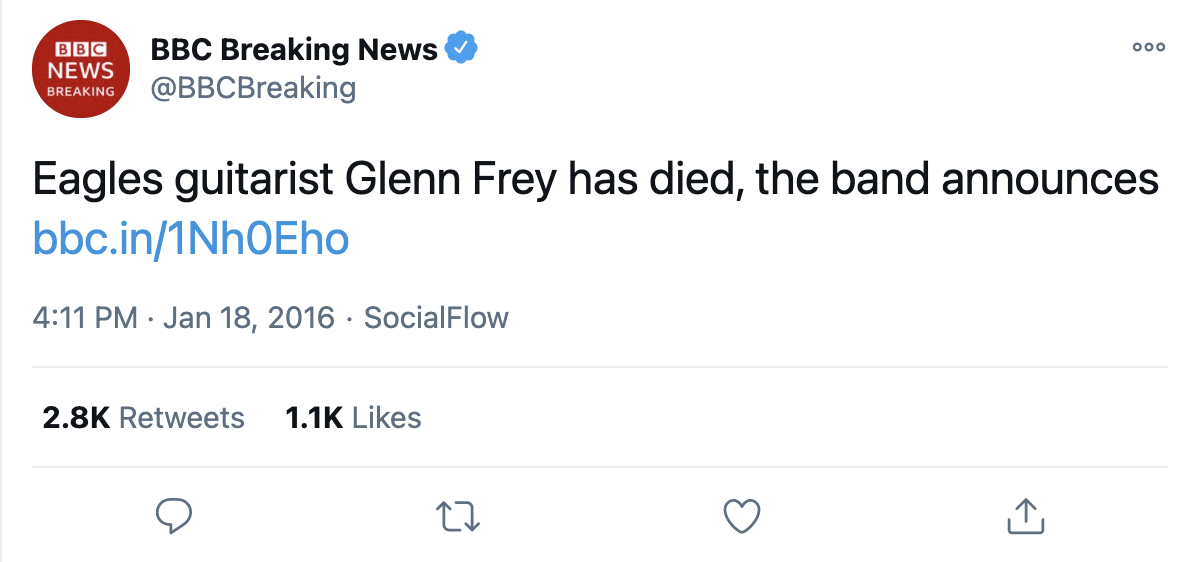
\includegraphics[width=9cm]{BBC Eagles.png}
    \caption{BBC Breaking Tweet}
    \label{fig:BBC Breaking Tweet, Jan 18, 2016}
\end{figure}
That tweet is also marked as a "rumor", even though it was not only true but from a reputable source. This data set does not differentiate between reputable and disreputable sources, nor does it do any post-hoc validation. This makes the truth values for this set highly problematic, and makes all of the RNN analyses off of this set equally untrustworthy. This thesis therefore discards the results of \citep{liu2018early,ma2017detect,ma2016detecting,khoo2020interpretable,liu2019early,huang2019deep} in terms of classification of fake news. This thesis therefore rejects the $\tau'$ values provided by this set.

Third, it has a disproportionately high number of users who are verified ($v = 1$). Twitter's requirements for being a verified account require follower count in the top 0.1\% of active accounts in a particular region or proof of being an important person off of twitter, such as being a professional artist/athlete, elected official, etc. \citep{twitter2020verified}; however, 1.4\% of the users in this set are verified. If verified is used as a quick stand-in for hub node, there are 14 times more hub nodes than would be expected in a random sample of twitter users. At the same time, there may be more verified users than necessary hub nodes. Since the total number of verified users is 3,061 with 212,360 unverified in the \textit{Twitter15} data set, yet the Arapacio set proposed only 1,000 hub nodes out of a set of 50,000,000, it is likely that users who are necessary hubs and users who are verified are not equivalent sets. Instead, users who are necessary hubs are likely a subset of users who are verified. 

Fourth, it breaks down the retweet paths into ordered pairs $(u_i,j_i)$ with $u_i$ being the user retweeting and $j_i$ being a batched time interval which is correlated but not equal to the actual time the retweet was posted ($j_i \neq p_i$ as defined by equation \ref{j_i}). In order to make their data set more RNN friendly, each retweet path was batched and partitioned, so that the length of entire time series for each retweet path is unique, but the distance between intervals is equal \citep{shu2017fake}. Since $j$ is not dependent on a timestamp, plotting all tweet paths as $r$ vs. $j$ would appear to show all these tweets were posted at identical times. That is intuitively incorrect. 

This means that all time-series related analysis would eventually have to be adjusted in order to provide relevant insights when working with a live-streaming data set. That having been said, the time series related work should be considered directionally meaningful.

Because of this, this thesis will work primarily on the tweets holistically - since the goal of the thesis is to provide a framework to order tweets by importance of fact-checking, any post-hoc $\tau'$ value is irrelevant. The time values for each tweet are also not relevant as, intuitively, $p_i \neq p_j$ for most tweets. However, $j$ is a meaningful stand-in as it will allow periods of time to be compared between tweets posted at different times. 

\subsection{User Data}
However, on the whole, this set matches much of the previous analysis. When plotting the $Y$ and $Z$ on a $\log_{10}$ scale (fig. \ref{fig:Twitter15 Follower}, fig. \ref{fig:Twitter15 Following}), the distribution is relatively normal and the power law (equation \ref{powerlaw}) holds true here:  $\gamma_{in} = 2.6$ and $\gamma_{out} = 1.62$. This is quite close to the $\gamma_{in}$ and the $\gamma_{out}$  from the Arapacio data set, 2.2 and 1.9 respectively.
 
 \begin{figure}[h]
\minipage{0.5\textwidth}
  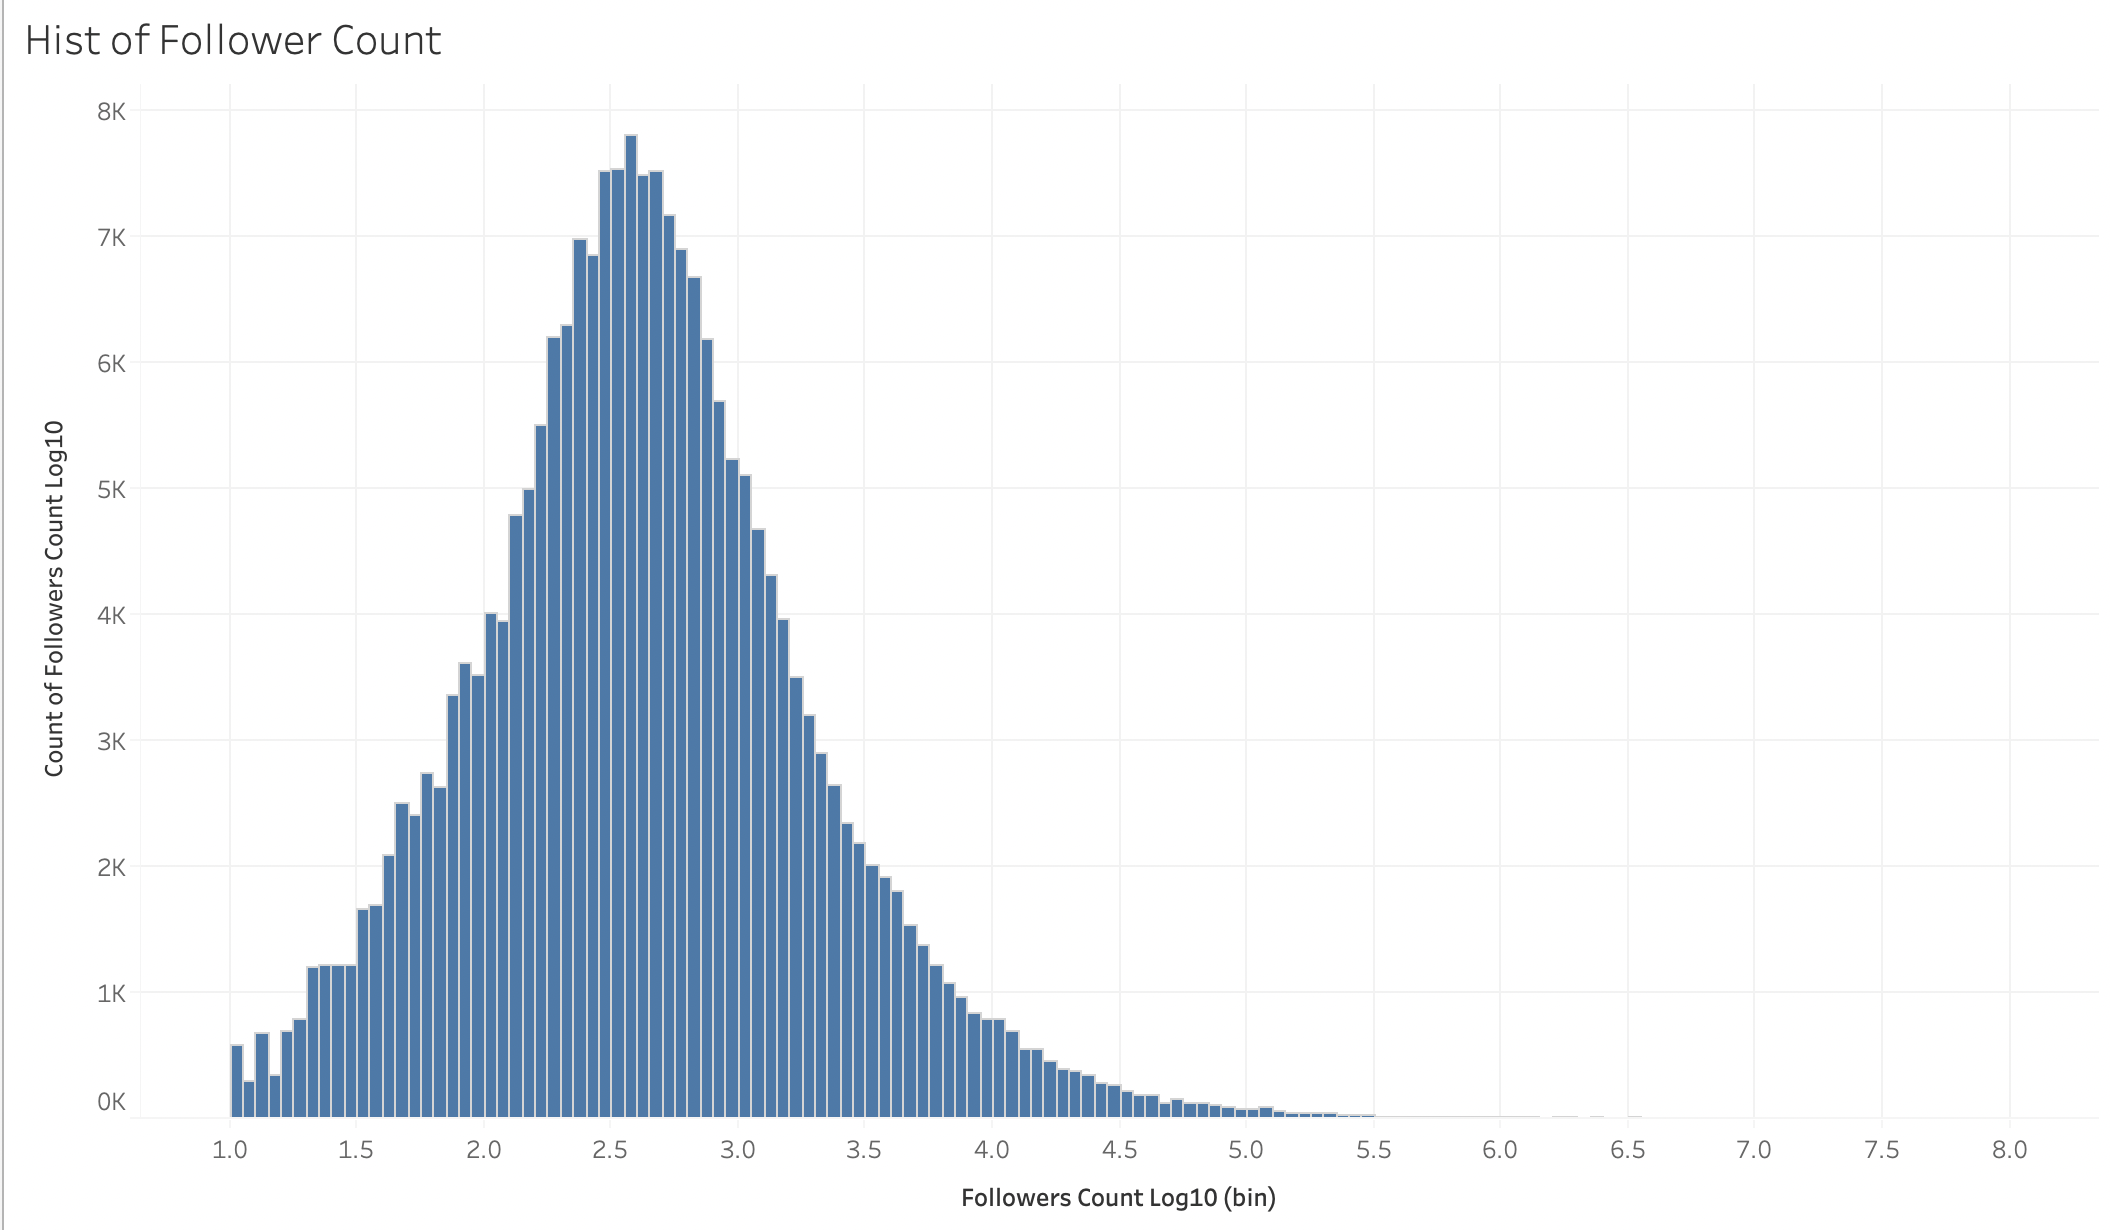
\includegraphics[width=\linewidth]{Twitter15 Follower Count.png}
  \caption{Follower Count, $|Z|$, for Twitter15 Set}\label{fig:Twitter15 Follower}
\endminipage\hfill
\minipage{0.5\textwidth}
  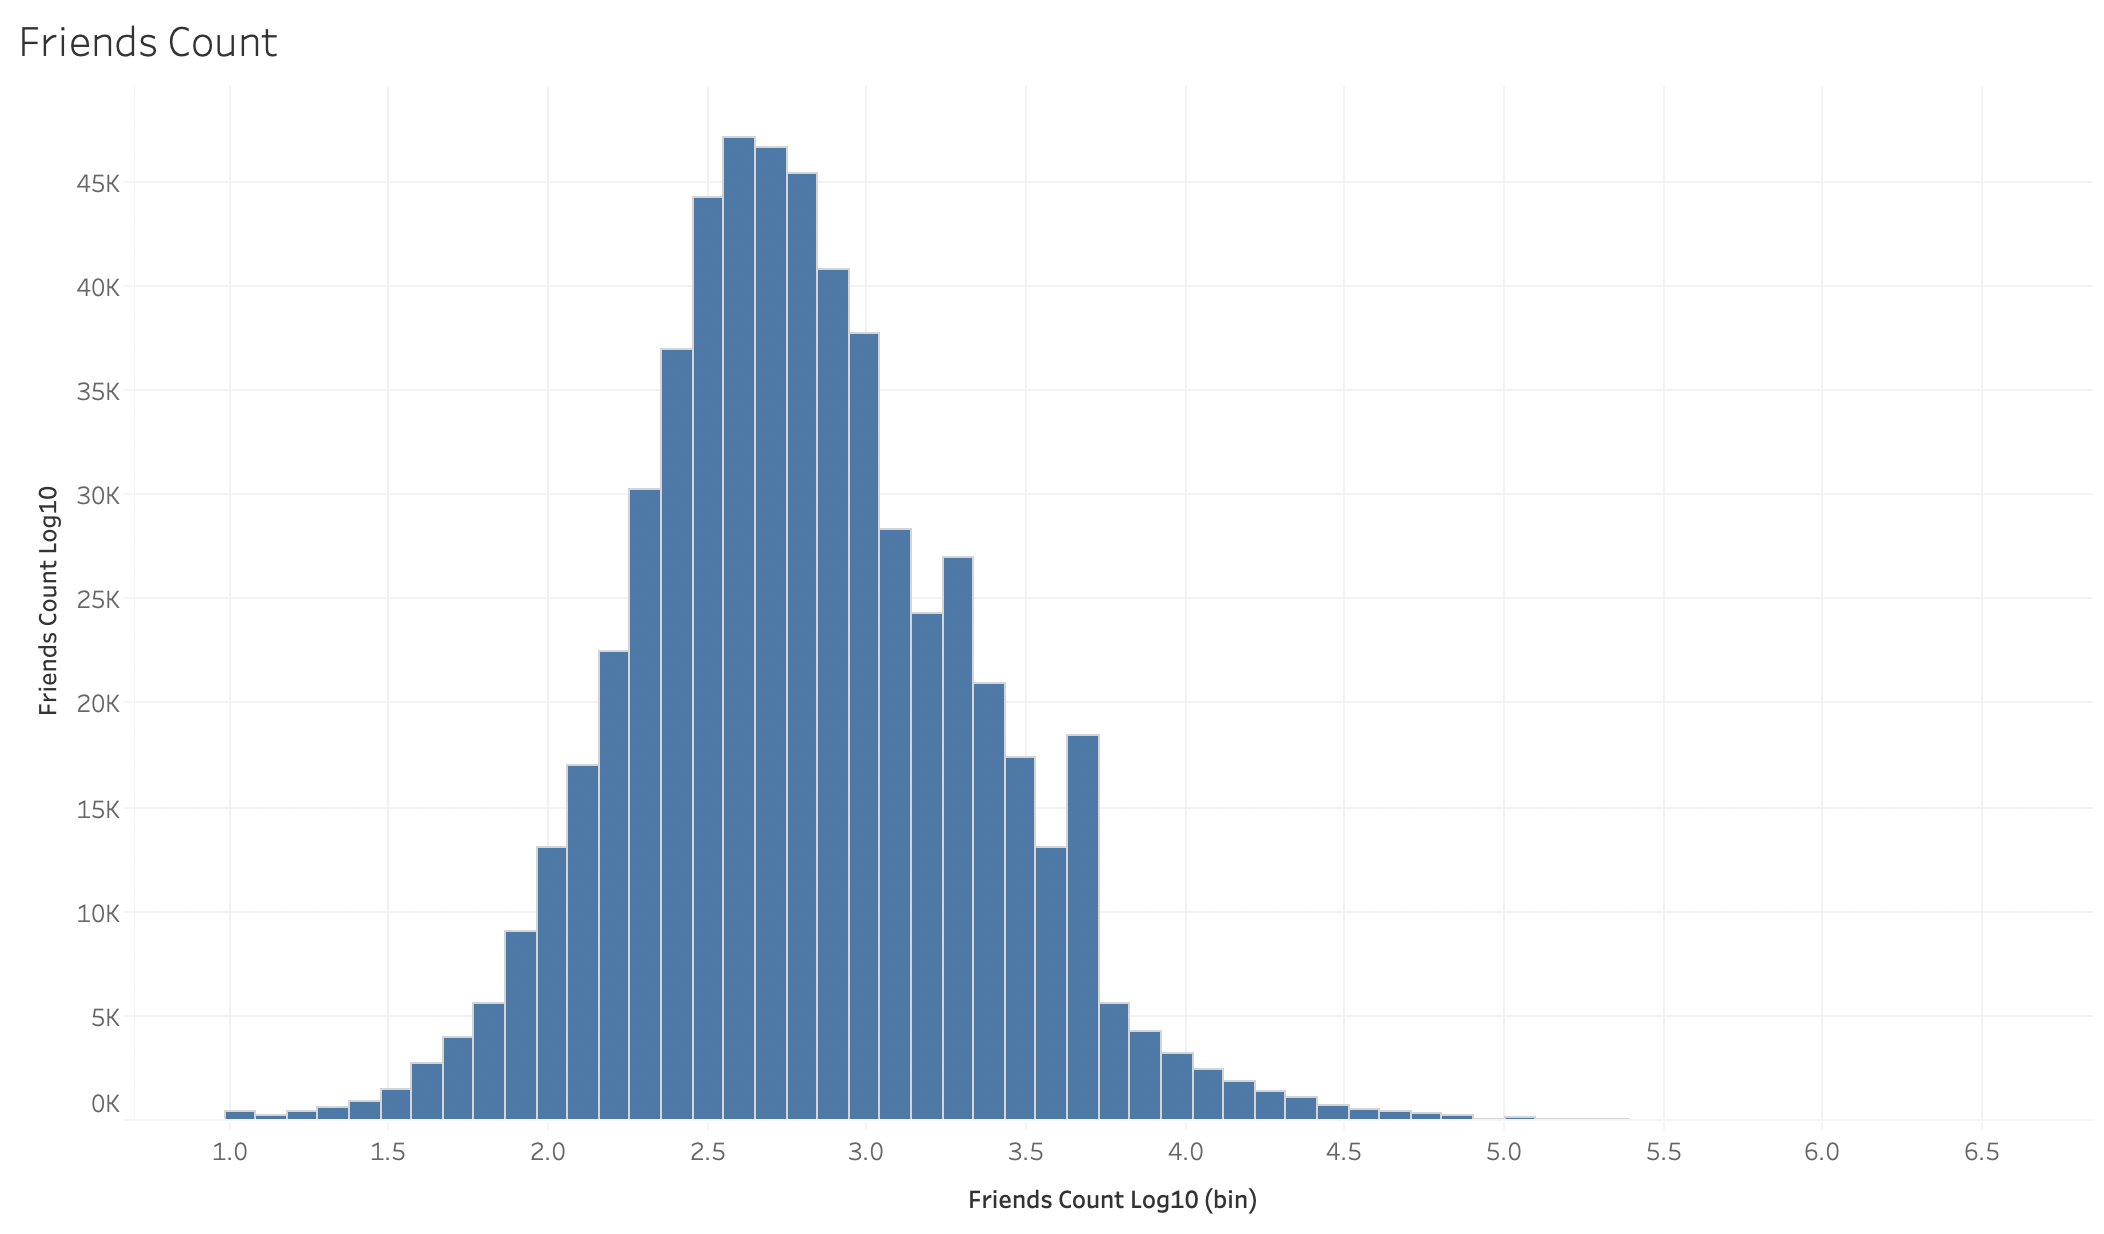
\includegraphics[width=\linewidth]{Twitter15 FriendsCount.png}
  \caption{Following Counts, $|Y|$, for Twitter15}\label{fig:Twitter15 Following}
\endminipage\hfill
\end{figure}



If the verified binary, $v \in \{0,1\}$, is a stand-in for hub nodes in this set, even though it is overly generous as discussed earlier, then non-hub nodes are close to the Arapacio numbers but hub nodes have an even greater $\phi$ than in the Arapacio set: $\forall \ u_n| v_n = 0:\langle |Y_n| \rangle \leq 400, \langle |Z_n| \rangle \leq 500, \langle  \phi_n \rangle \approx \frac{4}{5}$ and $\forall \ u_n| v_n = 1:\langle |Y_n| \rangle \leq 18,000, \langle |Z_n| \rangle \leq 1,300, \langle  \phi_n \rangle \approx 13.8$. 13.8 is clearly much greater than $\frac{7}{10}$; this could be due to the time the sample was collected as the Arapacio set was collected in 2009. The Twitter15 set contains, for example, former President Barack Obama, whose account has over 110M followers. 

Regardless, this set meets the requirements of a scale free network, and therefore all previously analyzed equations, such as equations \ref{Ldotpartisan} and \ref{echo chamber by followers} will be applied here.

\subsection{Retweets}
The retweet data, as mentioned earlier, is a vector of ordered pairs of users and time intervals so that $\vec{r}_i:\{(u_1,z_1), \cdots, (u_n,z_n)\}, t_i \in T$.

The total number unique users retweeting each tweet in the set is illustrated in fig. \ref{fig:Unique Retweeters}, and has the following properties as described in table \ref{Retweet Unique User Counts}:
\begin{figure}[h]
 \centering
  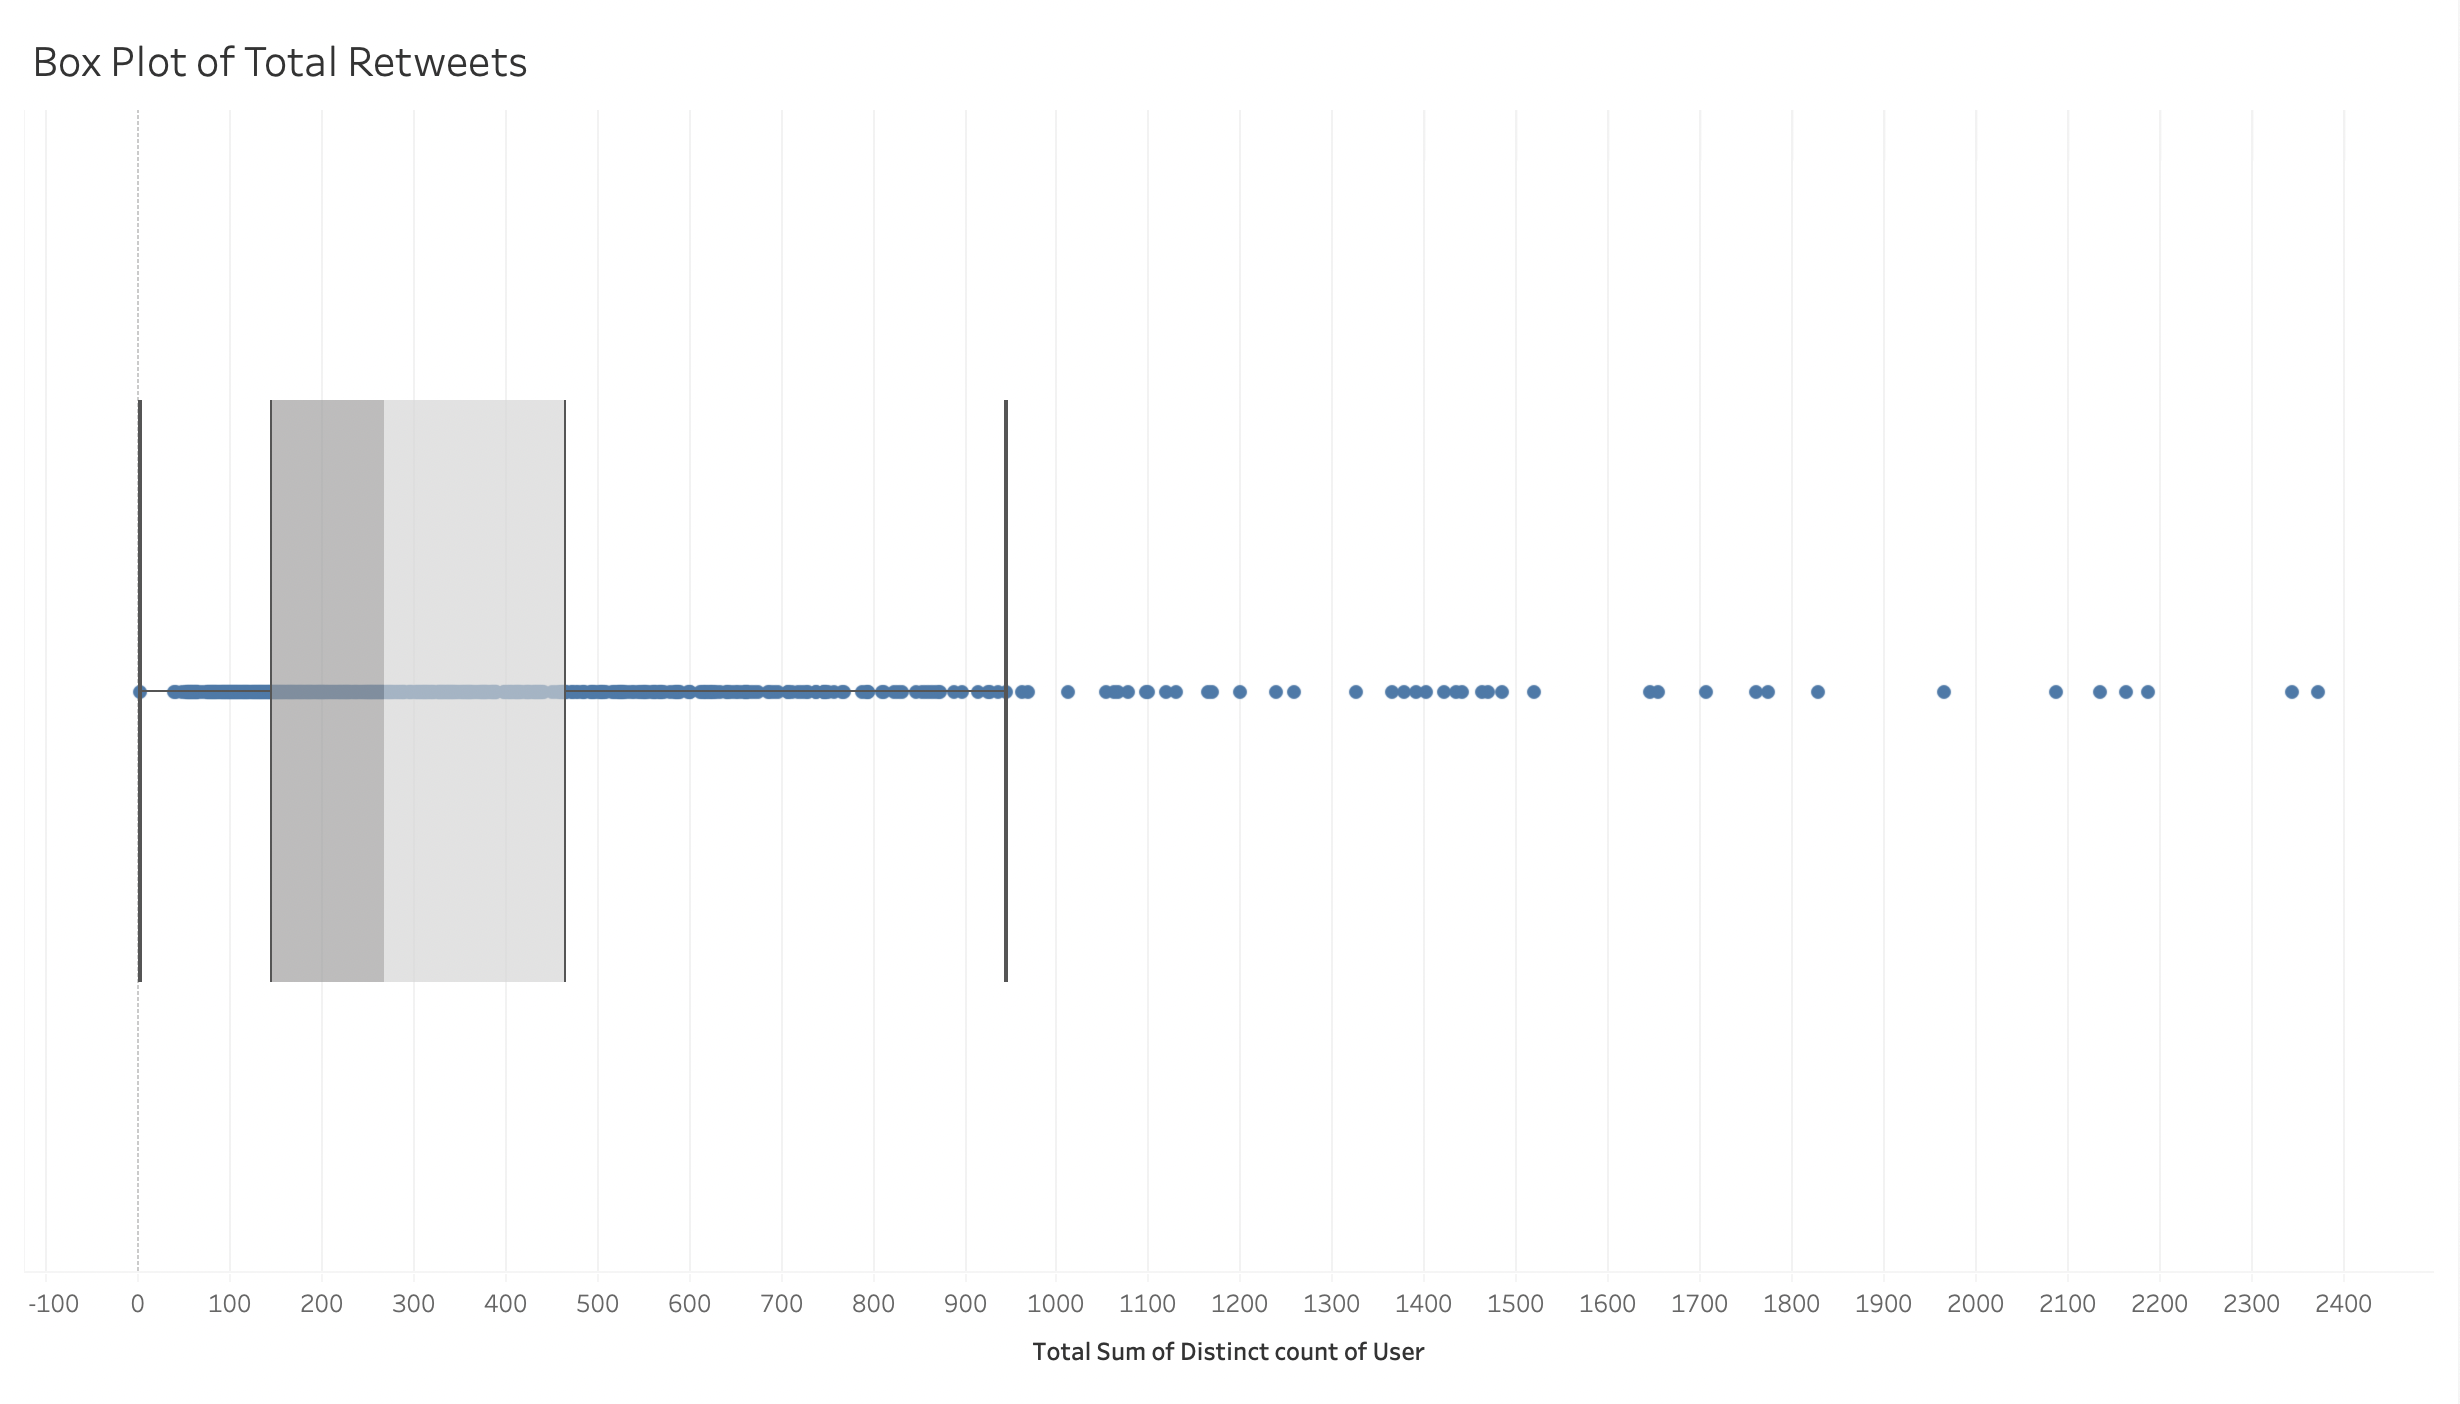
\includegraphics[width=12cm]{Retweet Box Plot.png}
  \caption{Box Plot of Unique Users Retweeting Each Tweet in the Data Set}\label{fig:Unique Retweeters}
 \end{figure}
 
\begin{table}[h]
\centering
\begin{tabular}{ |p{3cm}|p{3cm}|  }
\hline
\multicolumn{2}{|c|}{Retweet Unique User Counts} \\
\hline
Lower Whisker & 2\\
Lower Hinge & 146 \\
Median & 267.5 \\
Upper Hinge & 465.5 \\
Upper Whisker & 945 \\
\hline
\end{tabular}
\caption{Retweet Unique User Counts}
\label{Retweet Unique User Counts}
\end{table}

 
A graph of the running total of the number of unique users who have retweeted a particular tweet in figure \ref{fig:Users CumSum/Time} shows that the relationship is clearly logarithmic.The graph is set to a maximum $z = 24$ as one of the goals of this thesis is to rapidly identify tweets that need to be flagged for verification.
\begin{figure}[h!]
 \centering
  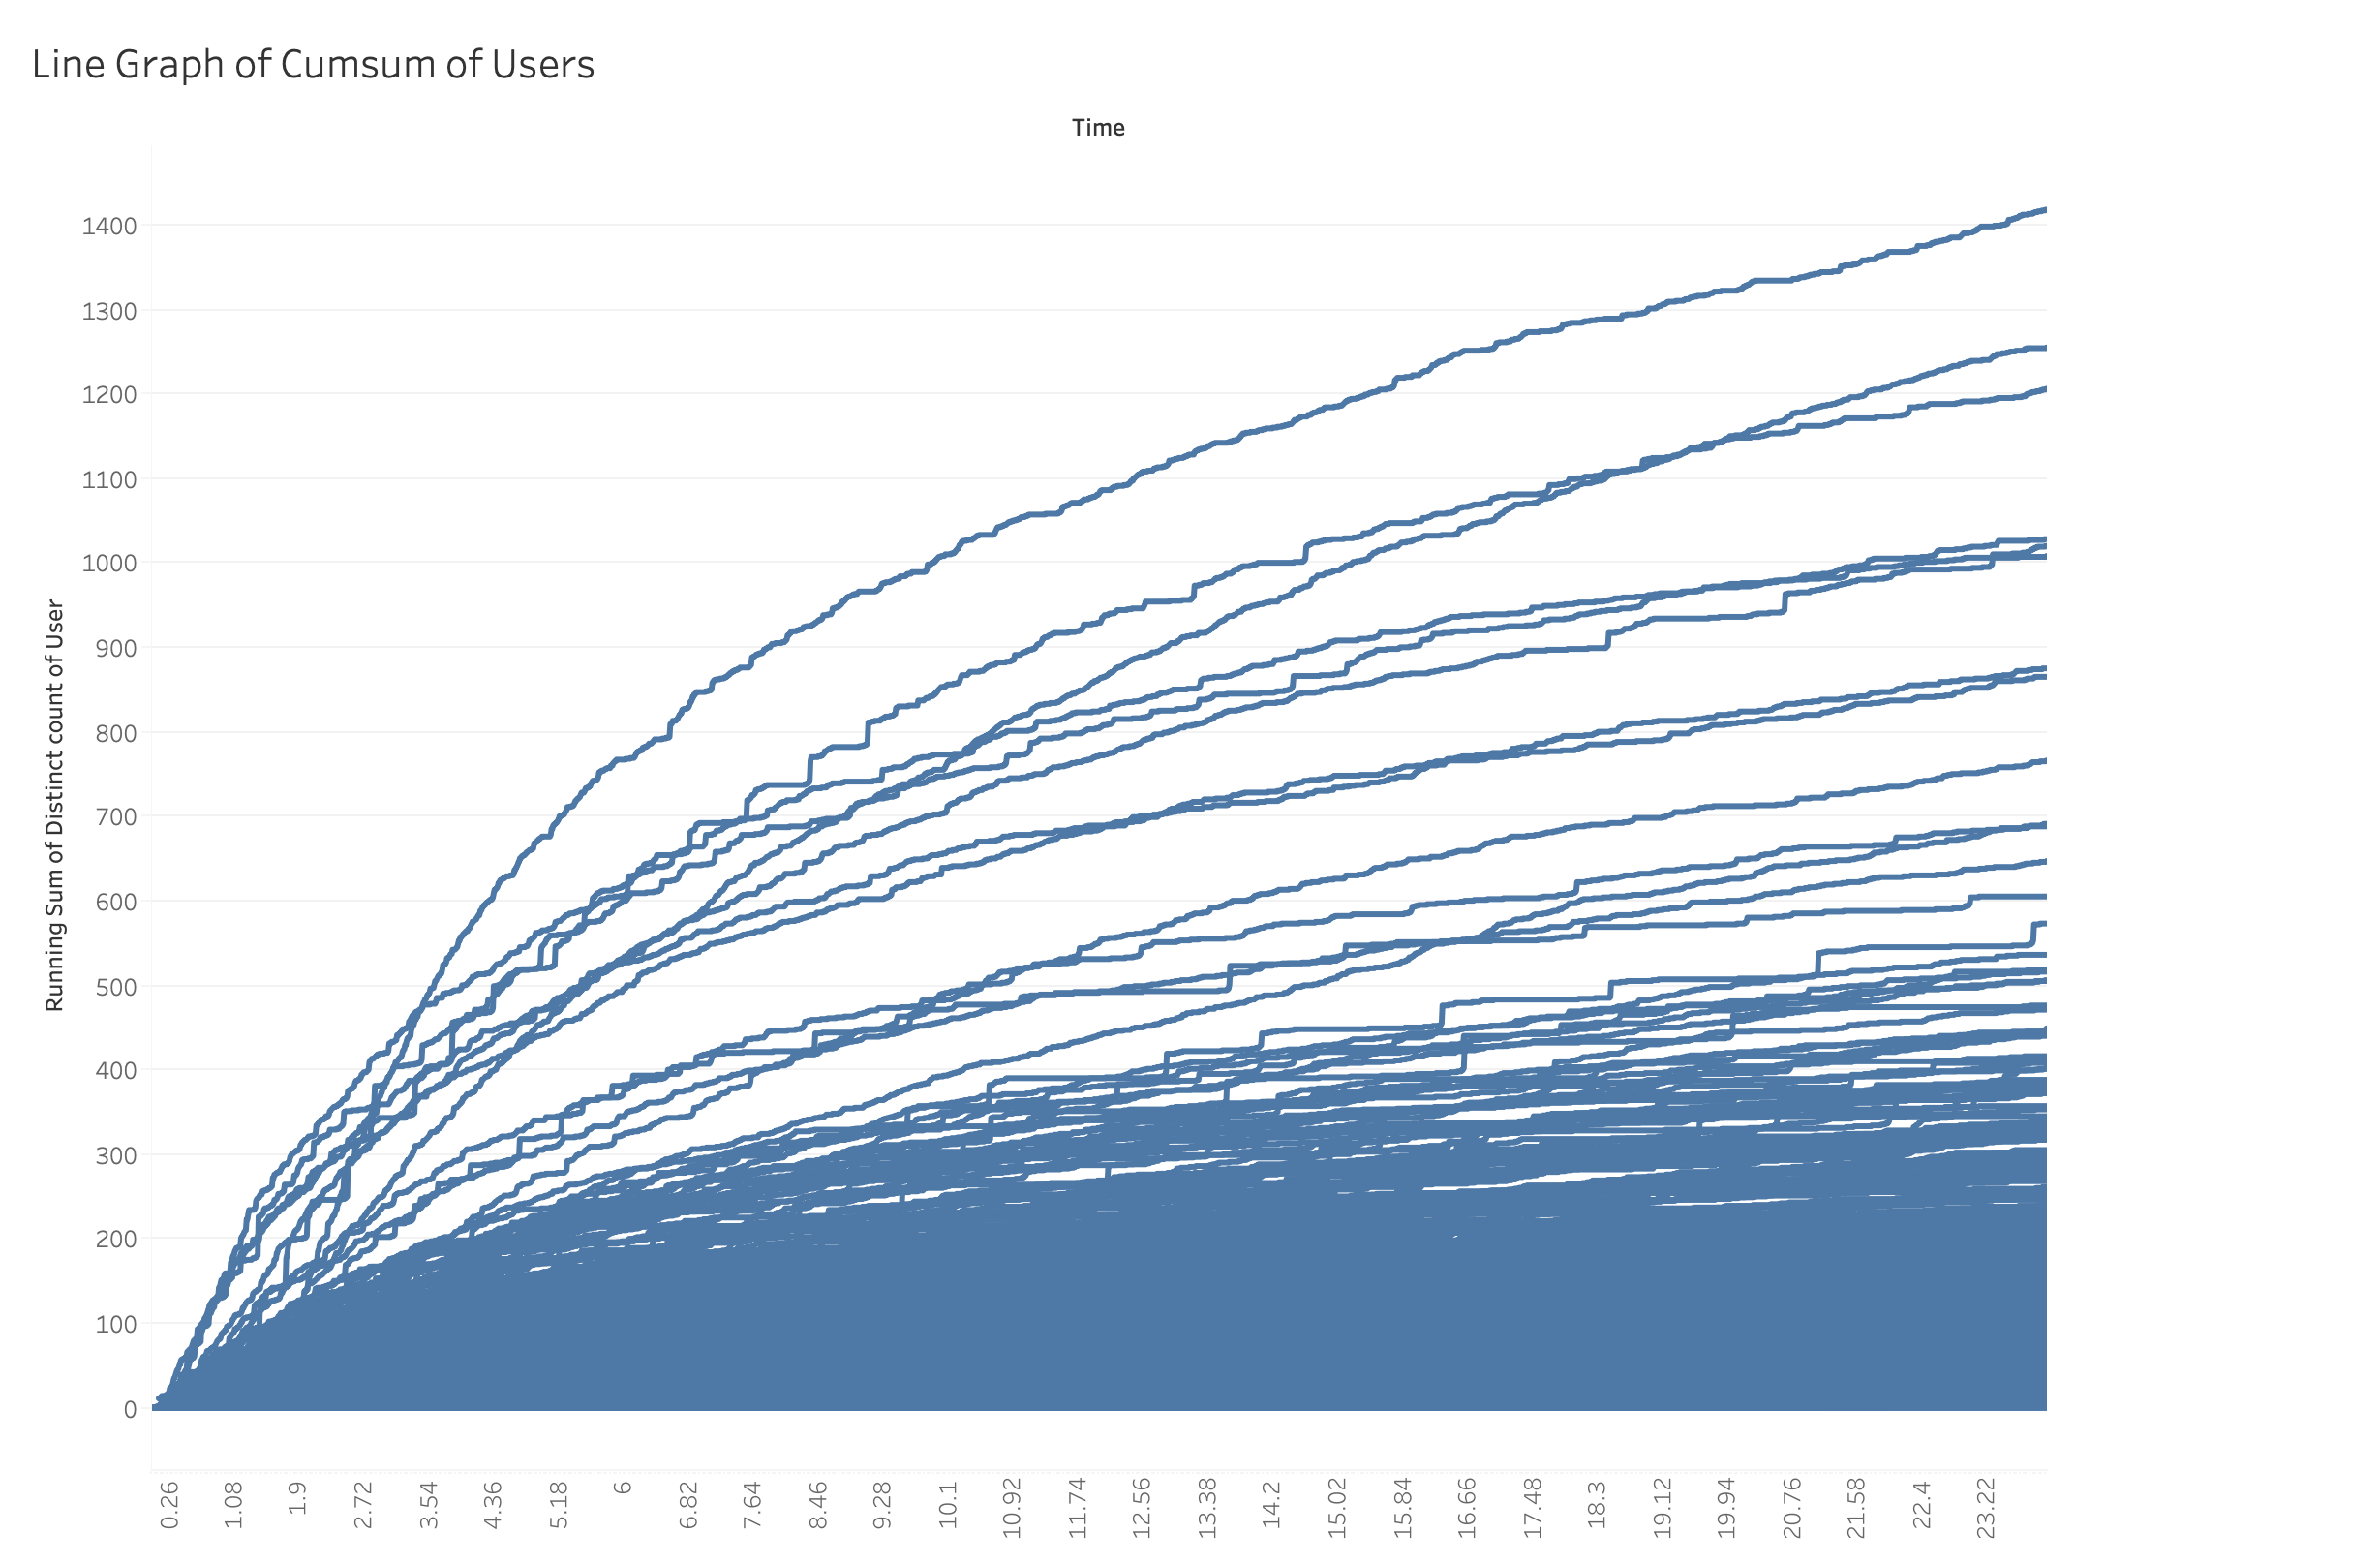
\includegraphics[width=12cm]{Linegraph cumsum users.png}
  \caption{Line Graph of Cumulative Sum of Retweeters over Time}\label{fig:Users CumSum/Time}
 \end{figure}

With simple regression to calculate the cumulative number of unique users retweeting a tweet to an $a\ln(j)$ equation with an intercept of zero (the intercept is manually forced to 0 as no tweet has $\geq 1$ retweet when time is 0) the number of the 680 tweets that fell into each statistical relevancy set as in the table \ref{Natural Log Fit}. The N/A values come from tweets that were insufficiently retweeted (1 or fewer retweets).   
\begin{table}[h!]
\centering
\begin{tabular}{ |p{3cm}|p{3cm}|  }
\hline
\multicolumn{2}{|c|}{$p$ value for $a\ln(j)$} \\
\hline
$p < 0.05$  & 654\\
$N/A$ & 18 \\
$ p \geq 0.05$ & 8 \\
\hline
\end{tabular}
\caption{$a\ln(z)$ fit}
\label{Natural Log Fit}
\end{table}

For an average tweet, the cumulative number of users at can be described by the equation $f(j)=85.8\ln(j)$, which has a $p$-value $<< 0.05$. This thesis will therefore accept that the distribution of the cumulative number of unique users retweeting an article has a natural log relationship to the amount of time that has passed.

It is also interesting to note the number of tweets with an $a > 85.8$ as seen in table \ref{a > 85.58}. Slightly less than 10\% of all tweets tracked showed a higher $a$ value than the average tweet.
\begin{table}[h!]
\centering
\begin{tabular}{ |p{3cm}|p{3cm}|  }
\hline
\multicolumn{2}{|c|}{Number of retweet paths with $a$ value relative to $\langle a \rangle$} \\
\hline
$a > 85.8$  & 67\\
$N/A$ & 18 \\
$ a \leq 85.8$ & 595 \\
\hline
\end{tabular}
\caption{Number of retweet paths with $a$ value relative to $\langle a \rangle$}
\label{a > 85.58}
\end{table}

This means that given the equation for cumulative users, $f(j) = a \ln(j)$, then the expected increase in users as a measure of time since the first post would be 
\begin{equation}
\label{rate of transmission}
    f'(j) = \frac{a}{j} 
\end{equation}
This $f'$ equation can be seen as the variable rate of transmission, typically referred to as an $r$ number in viral spread studies, but referred to as $\lambda$ in network theory. 
\subsection{Critical Rate of Transmission: $\lambda_c$}

Given the density equation for infected nodes $d$: \begin{equation}
    \label{densityequation}
    d \sim \exp\left(\frac{ - C}{\lambda}\right)
\end{equation} where $C$ is a constant and $\lambda$ is the rate of transmission \citep{pastor2001epidemic} (note that $d$ does not scale with the number of nodes in the network, which is typical of epidemics studied in previous literature \citep{marro2005nonequilibrium}), equation \ref{rate of transmission} can be merged in to provide:
\begin{equation}
    d \sim \exp\left(\frac{ - C}{a}j\right)
\end{equation}


The dynamic mean-field reaction rate from \citep{marro2005nonequilibrium} as relates to $j$ for a node with $k$ connections is: 
\begin{equation}
\label{dynamic mean-field reaction rate}
    \partial_jd_k(j) = - d_k(j) + \lambda k \big(1 - d_k(j)\big)\Theta(\lambda)
\end{equation}
In the case of twitter, $k$ is not the appropriate measurement, as $k$ is a directional-agnostic metric, whereas $\psi$ is directional. Indeed, both twitter and facebook's algorithms filter to content created by users the user in question follows. Therefore $k$ will be replaced with $\psi_{in}$, which measures only inbound connections. For legibility, let $\psi$ only refer to $\psi_{in}$ for this section.

\begin{equation}
\label{dynamic mean-field reaction rate}
    \partial_jd_{\psi}(j) = - d_{\psi}(j) + \lambda \psi \big(1 - d_{\psi}(j)\big)\Theta(\lambda)
\end{equation}

The probability that any particular node follows a user who shares misinformation, $\Theta(\lambda)$, is directly related to equation \ref{Pdotpartisan}:
\begin{equation}
\label{probability of infected node}
    \Theta(\lambda) = \sum_{\psi} \frac{\psi P(\psi)d_{\psi}\langle\rho_{\Delta}\rangle}{\langle \psi \rangle (0.5)}
\end{equation}

By setting the mean field equation, equation \ref{dynamic mean-field reaction rate}, set to a static state ($\partial_jd_{\psi}(j) = 0$), the $d_{\psi}$ can be solved for:
\begin{equation}
\label{static d_{\psi}}
    d_{\psi} = \frac{\lambda \ \psi \ \Theta}{1 + \lambda \ \psi \ \Theta}
\end{equation}

Substituting this into equation \ref{probability of infected node} provides:
\begin{equation}
    \Theta =  \frac{\sum_{\psi} \psi P(\psi)\langle\rho_{\Delta}\rangle}{\langle \psi \rangle(0.5)}\cdot \frac{\lambda \ \psi \ \Theta}{1 + \lambda \ \psi \ \Theta}
\end{equation}

$\Theta$ clearly must be between 0 and 1, inclusive, with the $\lambda$ value that sets $\Theta = 1$ called the critical $\lambda$ value or $\lambda_c$. The critical value is that where the network will be completely overrun and every node will be infected: 

\begin{equation}
\label{critical value equation}
    \frac{\sum_{\psi} \psiP(\psi)\langle\rho_{\Delta}\rangle\lambda_c\psi}{\langle \psi \rangle(0.5)} = \frac{\langle \psi^2 \rangle\langle\rho_{\Delta}\rangle}{\langle \psi \rangle(0.5)}\lambda_c = 1 \Rightarrow \lambda_c = \frac{\langle \psi \rangle(0.5)}{\langle \psi^2 \rangle\langle\rho_{\Delta}\rangle}
\end{equation}

For this data set, let $\langle \rho_{\Delta} \rangle = 0.5$. Much of the content in this set is non-partisan in nature, such as the ESPN and BBC tweets shared earlier. This allows for the $\left(\frac{0.5}{\rho_{\Delta}}\right)$ to cancel out, which is appropriate -- it is unlikely that an individuals political beliefs will shape their beliefs on whether or not Connor McGregor won a fight on a particular day. In general, the inclusion of $\rho$ is meaningful: by continuing with the viral spread metaphor, users with a $\rho_{\Delta} > 0.5$ are more likely to be immune from a particular strain of misinformation than those with  $\rho_{\Delta} < 0.5$.

With $\langle \rho_{\Delta} \rangle = 0.5$, $\lambda_c = \frac{434.6662}{9,117,302}=4.767487\times 10^{-5}$. This result is meaningful and a good predictor for this set, as the cumulative sum retweet paths (fig. \ref{fig:Users CumSum/Time}) follow a natural log shape line. Graphs like this have a very steep $f'$ before approaching $f' = 0$ as $j$ surpasses $a$. 

The seemingly low $\lambda_c$ value also illustrates how many tweets reach their maximum number of retweets quickly. In a 2018 analysis of over 700 million tweets, Mention discovered that while the mean number of retweets is 1696, the median is 0 \citep{mention2018twitter}. This shows just how skewed retweet values are: much like with the network equations earlier in this thesis, a small set dominate the network.

Given how steep $f'$ is for very small values of $j$, it is important to set a minimum threshold $j \geq 5$. This allows for the ability of a small number of people to retweet in rapid succession before the tweet reaches $j > a$. Otherwise, every tweet that is retweeted within a few seconds of creation could be flagged as $\lambda > \lambda_c$ when, in fact, it is not.

Therefore $\alpha_1$, the first metric for optimization, is:
\begin{equation}
    \label{alpha1}
    \alpha_1 = \frac{\lambda}{\lambda_c}, j\geq 5
\end{equation}

\subsection{Fraction of Users to Target}
In immunization work on network theory \citep{pastor2002immunization}, the fraction of individuals that should be vaccinated in a targeted scenario, $v$, is equal to 
\begin{equation}
    v = \sum_{k > k_t}P(k)
\end{equation}
where $k_t$ is a minimum threshold of connections and any user with connections above that threshold will be vaccinated. 

Combined with \ref{Pdotpartisan}:
\begin{equation}
\label{probability of vaccinated}
p(v) = \frac{\sum_{k>k_t(v)}kP(k)\langle \rho_{\Delta_{k>k_t}}\rangle}{\sum_{k}kP(k)\rho_{\Delta}}
\end{equation}

If those people are considered removed, then the new distribution would be \citep{cohen2001breakdown}:
\begin{equation}
    P_v(k) = \sum_{1\geq k}^{k_t}P(q)\binom{q}{k}(1-p)^kp^{q-k}
\end{equation}
This leads to new $\langle k \rangle_v$ and $\langle k^2 \rangle_v$ values (after cut-off introduction and link removals)\citep{pastor2002immunization}: 
\begin{align*}
        \langle k \rangle_v &= \langle k \rangle_t(1-p)\\
         \langle k^2 \rangle_v &= \langle k^2 \rangle_t(1-p)^2+\langle k \rangle_t\ p(1-p)
\end{align*}

At this point, $k$ can be replaced with $\psi$ (as before, only referring to inbound connections here) to make it compatible with equation \ref{critical value equation} to determine $v_c$, the critical fraction of users who need to be vaccinated:
\begin{equation}
\label{v_c equation}
 \frac{\langle \psi^2 \rangle_{v_c}\langle\rho_{\Delta}\rangle}{\langle \psi \rangle_{v_c}(0.5)} \equiv \frac{\langle \psi^2 \rangle_{t}\langle\rho_{\Delta_t}\rangle}{\langle \psi \rangle_{t}(0.5)}(1-p(v_c))+p(v_c)=\lambda^{-1}\frac{\rho_{\Delta_t}}{0.5}
\end{equation}

To determine a more actionable $v_c$, $v$ can be rewritten as an integral starting at 1 as, even though users can have no followers, those are not relevant to our analysis as they have no possibility of infecting others (furthermore, they are likely to be bots or spam, which should be removed from the set per the section on \textit{synthetic a priori} analysis:
\begin{equation}
\begin{split}
    v & = 1 - \int_1^{\psi_{t}} P(\psi)d\psi \\
   v & = 1 - \int_1^{\psi_{t}} \psi^{-\gamma}d\psi \\
   v & = 1 - \left(\frac{\psi_{t}^{-\gamma +1}}{-\gamma+1}-\frac{1^{-\gamma +1}}{-\gamma+1}\right) \\
   v & = \frac{-\gamma+1 - \psi_{t}^{-\gamma +1} -  1^{-\gamma +1}}{-\gamma+1} \\
   v(-\gamma + 1) & = -\gamma - \psi_{t}^{-\gamma +1}\\
   -\big(v(-\gamma + 1) + \gamma\big) & = \psi_{t}^{-\gamma+1}\\\
   \big(-v(-\gamma + 1) - \gamma\big)^{\frac{1}{-\gamma + 1}} & = \psi_t
\end{split}
\end{equation}

As can be seen from this graph utilizing the $\gamma_{in} = 2.2$ as determined earlier:
\begin{figure}[h]
 \centering
  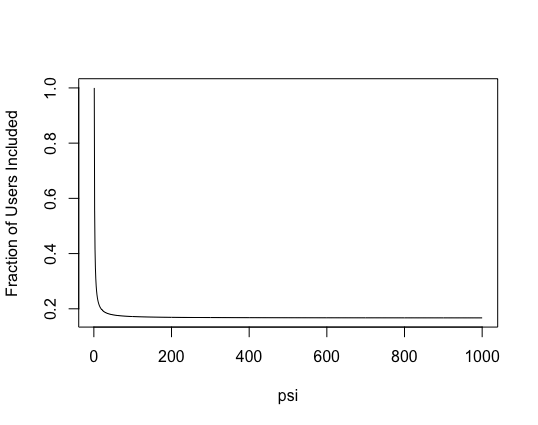
\includegraphics[width=10cm]{Fraction of users included.png}
  \caption{Fraction of users, $v$ vs. $\psi$}\label{fig:Fraction of users,v, vs. $\psi$}
 \end{figure}

$v \simeq \psi_t^{-2}$ as $\psi \rightarrow \infty$ with a $p$-value $<< 0.01$. This matches the generalized equation for BA models: $v = m^2k_t^{-2}$, where $m$ is the minimum number of connections any node in the model has (here $m = 1$) \citep{pastor2001epidemic}. This can then be manipulated to: $\psi_t \simeq v^{-1/2}$. 

This means that the probability of a random individual connected to a vaccinated node would be $p(v) = \sqrt{v}$. From there, $\langle \psi \rangle_t \simeq 2$, and $\langle \psi^2 \rangle_t \simeq 2 \ln(v^{-1/2})$, with $\psi_t = v^{-1/2} \rightarrow \infty$. This can be combined with equation \ref{v_c equation} to determine $v_c$, the critical fraction that needs to be vaccinated:
\begin{equation}
\label{reduced v_c} 
    v_c \simeq \exp{(-2/\lambda)}
\end{equation}

This equation has  been applied to examples such as viruses in the internet \citep{kephart1993computers}, STI transmission \citep{anderson1992infectious,lloyd2001viruses}, and other epidemics \citep{diekmann2000mathematical}. 

By this point, it should come as no surprise that "vaccinated" and "fact-checked" are interchangeable for the context of this thesis. Equation \ref{reduced v_c} can be easily adapted for a variety of scenarios. It can be used with an average $\langle \lambda \rangle$ for all tweets to determine the threshold of tweets/users to fact-check; in a situation like conspiracies about forest fires being spread by Antifa \citep{robinson2020oregon}, $\lambda_i$ can be calculated for that particular topic and $v_c$ can be used to calculate the number of tweets that must be fact checked. Much like it's unnecessary to vaccinate every node during an epidemic in order for the disease to die out, it is similarly unnecessary to fact check all possible tweets in order for a thread of misinformation to die out.

Therefore, for the total set of $F$ and the subset of $F$ relating to topic $i$: 
\begin{equation}
    \label{size of F}
    \begin{split}
    |F| \leq v_{c}|T| \\
    |F_{i}| \leq v_{c,i}|F|
    \end{split}
\end{equation}
Since one of the goals is to minimize the size of $F$, equation \ref{size of F} can be used as a constraint with slack variables as needed.

For this dataset, using an average $\lambda$, $v_c \simeq \exp(-j/42.9)$, the graph of $v_c$ vs. $j$ is shown in fig. \ref{fig:v_c exp(-x/42.9)}. In order to see the more rapid 
\begin{figure}[h]
 \centering
  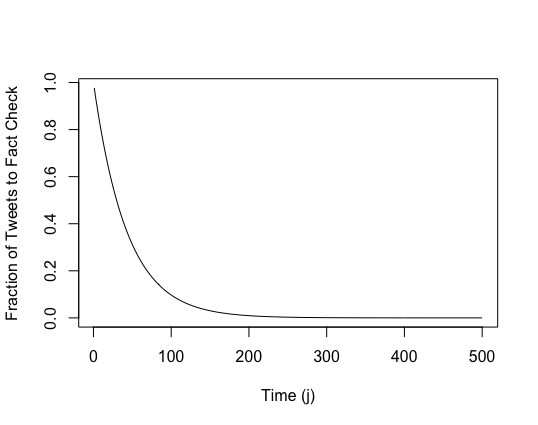
\includegraphics[width=10cm]{v_c e to the -x42.9.png}
  \caption{Fraction of tweets to fact check, $v_c$, vs. $j$}\label{fig:v_c exp(-x/42.9)}
 \end{figure}
 
 If $j \geq 5$, as proposed in the \ref{alpha1}, this means that the maximum number of tweets in $F$ would be:
\[
 \begin{split}
 |F| & \leq (v_c)(|T|) \\
  |F| & \leq \big(\exp(-j/42.9)\big)(680) \\
 |F| & \leq (0.90)(680) \\
  |F| & \leq612
 \end{split}
\]
However, by the time that $j$ reaches 20, the percent of tweets to validate drops from 90\% down to 62\%. 

\subsection{Topic Aggregation}
As alluded to in the previous section, users and tweets can be grouped into "topics" or subsets (i.e.  for topic $i$, $T_i \subset T$). This is not dissimilar to what Twitter currently does when it labels a topic as \textit{trending} (fig. \ref{img:Trending Topics}), with a key difference. 

\begin{figure}[htp]
    \centering
    
\includegraphics[width=6cm]{Twitter Trending.png}
    \caption{Trending Topics on Twitter, Jan 30 2020}
    \label{img:Trending Topics}
\end{figure}


Trending is based almost exclusively on kurtosis over increasingly small pieces of time \citep{dewey2015freddie,lotan2015freddie}. It is the opposite of the goal achieved with equation \ref{alpha1}, which attempts to remove spikes in traffic over a small period of time -- trending operates more akin to jerk in physics and is connected to the tweet velocity, $\omega$ from equation \ref{tweetvelocity} which is based off of retweets, rather than $\lambda$: 
\[
    \frac{\partial^2 \omega}{\partial j^2}
\]

There are two flaws here. First, using $r$ over $\lambda$ favors topics that may or may not quickly expire on their own while ignoring slowly growing topics. In the Washington Post article cited earlier, \#FreddieGray was never considered trending on Twitter even though the story was featured prominently on CNN, ABC, the New York Times, etc. and more than 150,000 people tweeted on the topic on April 25, 2015 (fig. \ref{img:Trendinalia 2015})
\begin{figure}[htp]
    \centering
    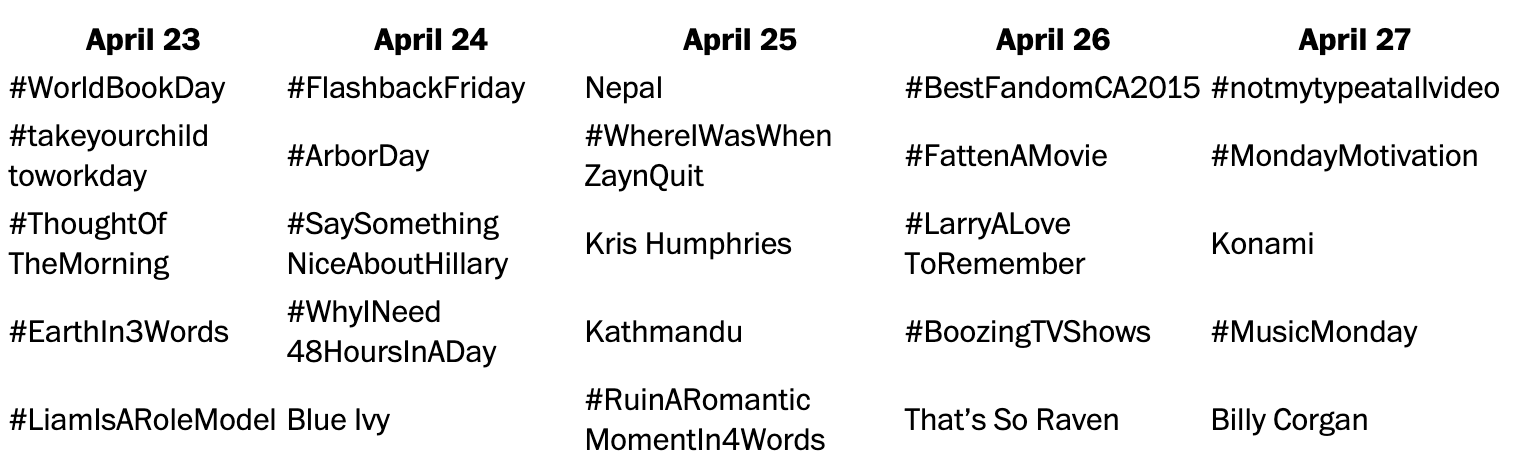
\includegraphics[width=11cm]{Trendinalia Apr, 2015.png}
    \caption{Trending Topics on Twitter via Trendinalia, Apr 2015}
    \label{img:Trendinalia 2015}
\end{figure}
. 

As Lotan, a data scientist for Buzzfeed, pointed out:
\begin{displayquote}
1. The longer a term stays in the trending topic list, the higher velocity [of tweets] required to keep it there. \\
2. It is much easier for a term never seen before to become a Twitter trend, and finally \\
3. It is extremely important to understand what else is happening in the region or network (if Kim Kardashian’s show is airing, you can forget about trending!).
\end{displayquote}

Sociologist Zeynep Tufekci argues in multiple media that this becomes de-facto censorship \citep{tufekci2017twitter,tufecki2018democracy,tufekci2017we,tufekci2014online}. She provides numerous examples, such as Facebook's 2014 trending window which provided high visibility to topics such as the "Ice Bucket Challenge", but completely left off the protests in Ferguson, MO after the shooting of Michael Brown. This, she contends, creates effective censorship: by denying visibility to a particular topic while elevating another, social media is making (whether intentional or not) editorial decisions. 

In defense of utilizing $\frac{\partial^2 \omega}{\partial j^2}$ to determine whether or not a topic is trending, a high value here shows very high engagement at a particular point in time: there is nothing inherently wrong or immoral about connecting disparate groups who are all watching and commenting on a TV show at the same time. At the same time, as both Tufecki and Lotan point out, it's easy for important topics to get drowned out by noise.

 %The usage of $\frac{\lambda}{\lambda_c}$ resolves this issue. Every tweet has a $\lambda$ value, as illustrated in equation \ref{rate of transmission}, which can be compared to the critical rate of transmission. 

Indeed, a superior way to determine if a topic is trending for the purposes of misinformation discovery, instead of comparing $\langle \omega_i \rangle$ vs $\langle \omega \rangle$ is to compare $\langle \lambda_i \rangle$ vs. $\langle \lambda \rangle$. Since $j$ is a constant value at the point of comparison, a unique point in time, the equation \[\frac{\partial^2 \lambda_i}
{\partial^2 \langle \lambda \rangle}\] is correct for determining if a particular topic is trending at a unique value of $j$. By using this equation, especially setting $j \geq 5$ as in equation \ref{alpha1}, small arbitrary topics that peak early in terms of total retweets do not make it into $F$:
\begin{equation}
    \label{Trending}
    T_i \subset F \subset T: \partial^2 \langle \lambda_i \rangle > \partial^2 \langle \lambda \rangle, j \geq 5
\end{equation}

There is no need to replace the underlying algorithm for topics that are trending, which is presumably a mixture of NLP and an RNN, as it is already an effective and sustainable solution. 



\section{Situations where $\rho_{\Delta} \neq 0.5$} 
Clearly, the \textit{Twitter15} data set is not representative of social media as a whole, even when examining $\lambda$ values. The tweet with the highest $\lambda$ marked "false", as it is an unverified rumor, is fig. \ref{img:Voldemort Tweet}. 
\begin{figure}[htp]
    \centering
    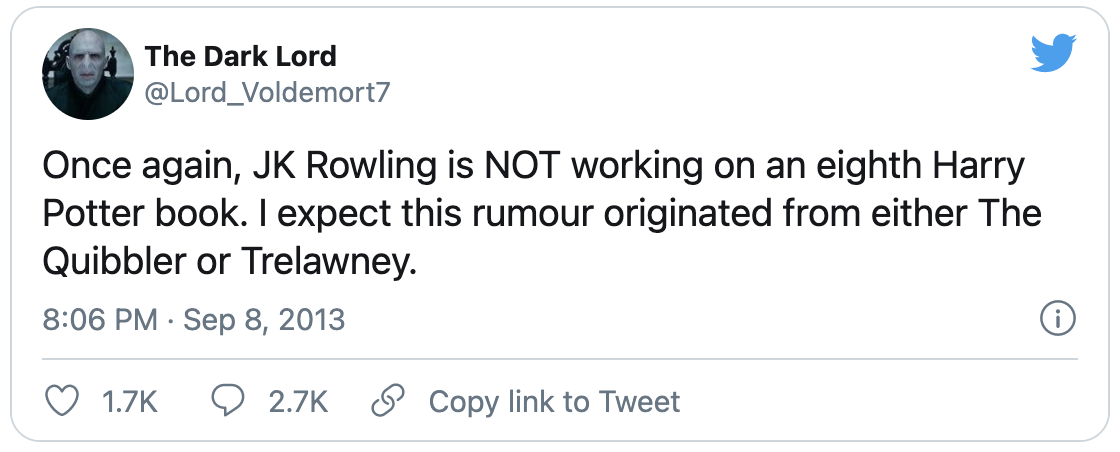
\includegraphics[width=8cm]{voldemort tweet.png}
    \caption{Tweet with the Highest $\lambda, j \geq 5$ in the \textit{Twitter15} Data Set}
    \label{img:Voldemort Tweet}
\end{figure} Much like with the other examples from this set, it fails every test provided in the section on the definitions of misinformation: there is no malice or intentionality nor an incitement to violence. There is no possibility that a person reading this tweet, no matter how strong of a Harry Potter fan they are, would be a threat to themselves or others. There is no emotional or existential call to action, there is no attempt to alter a debate on public policy, and there is no slander or libel. In short, if every user who follows this account read and believed this tweet, the ramifications would be effectively nonexistent. 

Therefore, it is important to examine sets where the partisanship is \textit{not} irrelevant: $\rho_{\Delta} \neq 0.5$. 
\subsection{Determining $\rho_{\Delta}$}
While this task may seem fruitless at first -- it would be an impossible task to determine a partisanship for every tweet in comparison to the partisanship of all users -- it actually makes the entire task easier. As shown in equations \ref{ech chamber}, \ref{peopletoextremes}, and \ref{echo chamber by followers}, an individual's partisanship is directly related to the partisanship of the most connected person in their network. While one might argue that an individual might follow opposing view points, the results of equation \ref{party overlap twitter} show that this is statistically unlikely to be the case for $p < 0.05$. Similarly, one might argue that merely following someone does not necessarily imply $\rho_i \simeq \rho^*$, where $i$ is the unique user and $\rho^*$ is the partisanship for $u^*$, the user with the $\max(|\psi|), u^* \in Z_i$. This thesis does not deny that. However, there are key points to recall:
\begin{enumerate}
    \item Users who follow $u^*$ are likely to follow other similar users with similar viewpoints (eq. \ref{Ldotpartisan}).
    \item The probability that an individual follows a user who shares misinformation is not changed by the individual's reaction to the misinformation (eq. \ref{probability of infected node}).
    \item Since this thesis focuses on modeling misinformation as viral spread, there is nothing incorrect with including users who may be "immune" to the misinformation as natural immunity also occurs in traditional viral spread (eq. \ref{reduced v_c}).
\end{enumerate}



\newpage
%%%%%%%%%%%%%%%%%%%%%%%
%% The bibliography

\bibliography{NETNbibsamp}

%\section{Technical Terms}

%\textbf{Technical Term} a key term that is mentioned in an NETN article and whose usage and definition may not be familiar across the broad readership of the journal. 

%\textbf{Technical Term} a key term that is mentioned in an NETN article and whose usage and definition may not be familiar across the broad readership of the journal. 

%\textbf{Technical Term} a key term that is mentioned in an NETN article and whose usage and definition may not be familiar across the broad readership of the journal. 

%\textbf{Technical Term} a key term that is mentioned in an NETN article and whose usage and definition may not be familiar across the broad readership of the journal. 


%% No appendices allowed in Network Neuroscience style
%\appendix

\end{document}
\pdfendlink
